\documentclass[diplomskirad]{fer}

% Language and encoding
\usepackage[utf8]{inputenc}
\usepackage{csquotes}

% Math and symbols
\usepackage{amsmath}
\usepackage{amsfonts}
\usepackage{amssymb}

% Graphics and figures
\usepackage{graphicx}
\usepackage{float}
\usepackage{subcaption}
\usepackage{tikz}
\usetikzlibrary{shapes,arrows,positioning,fit,backgrounds}

% Code listings
\usepackage{listings}
\usepackage{xcolor}

\renewcommand{\lstlistingname}{Primjer}

% Configure listings for proper diacritic handling
\lstset{
  basicstyle=\footnotesize\ttfamily,
  breaklines=true,
  xleftmargin=0.5cm,
  xrightmargin=0.5cm,
  frame=single,
  extendedchars=true,
  inputencoding=utf8,
  literate={č}{{\v{c}}}1 {ć}{{\'c}}1 {ž}{{\v{z}}}1 {š}{{\v{s}}}1 {đ}{{\dj}}1 
           {Č}{{\v{C}}}1 {Ć}{{\'C}}1 {Ž}{{\v{Z}}}1 {Š}{{\v{S}}}1 {Đ}{{\DJ}}1
}

% Hyperlinks
\usepackage{hyperref}
\hypersetup{
    colorlinks=true,
    linkcolor=blue,
    filecolor=magenta,
    urlcolor=cyan,
}

% Custom commands
\newcommand{\code}[1]{\texttt{#1}}
\newcommand{\system}{DCAT Metadata Analysis System}

% Set bibliography title in Croatian
\renewcommand{\bibname}{Literatura}

% Add bibliography and other lists to the table of contents
\usepackage{tocbibind}

% Thesis information (update as needed)
\title{Sustav za analizu meta podataka otvorenih skupova podataka}
\naslov{Sustav za analizu meta podataka otvorenih skupova podataka}
\brojrada{874}
\author{Luka Habuš}
\mentor{Igor Čavrak, izv. prof. dr. sc.}
\date{July 2025}
\datum{srpanj 2025.}

\begin{document}

% Title page
\maketitle

% Duplicate title page (identical to the first)
\maketitleHR{2}

% Thesis assignment (if available)
\zadatak{hr_0036517946_92.pdf}

% Acknowledgments (optional)
\begin{zahvale}
%  Ovdje upišite zahvale / Write in the acknowledgment
\end{zahvale}

% Start page numbering
\mainmatter

% Table of contents
\tableofcontents

% List of figures
\listoffigures

% Main chapters
\chapter{Uvod}
\label{ch:introduction_background}

\selectlanguage{croatian}

\section{Problemski okvir i motivacija}

U suvremenom digitalnom ekosustavu, otvoreni podaci predstavljaju fundamentalni resurs za unapređenje transparentnosti javne uprave, poticanje znanstvenih istraživanja i generiranje ekonomskih inovacija. Portali poput službenog EU Portala otvorenih podataka nude pristup milijunima skupova podataka koji obuhvaćaju širok spektar domena, od okoliša i energetike do zdravstva i ekonomije. Unatoč golemom intrinzičkom potencijalu, stvarna iskoristivost ovih resursa ostaje na relativno niskoj razini. Uzroci ovog nesrazmjera su višestruki i složeni.

Primarno, postoji tehnička barijera. Pretraživanje i dohvaćanje podataka s portala koji primjenjuju tehnologije semantičkog weba zahtijeva ovladavanje specifičnim upitnim jezicima, među kojima se ističe SPARQL. Navedeni jezik, unatoč svojoj izražajnoj moći, nije intuitivan za korisnike bez formalne tehničke naobrazbe, kao što su novinari, analitičari javnih politika ili studenti. Time se sužava krug potencijalnih korisnika otvorenih podataka.

Nadalje, uočava se nepreciznost tradicionalnih metoda pretrage. Većina postojećih portala implementira pretragu temeljenu na podudaranju ključnih riječi. Takav pristup često rezultira nerelevantnim ishodima jer ne posjeduje sposobnost razumijevanja semantičkog konteksta korisničkog upita. Primjerice, upit "utjecaj prometa na kvalitetu zraka u urbanim sredinama" može propustiti relevantne skupove podataka koji koriste semantički ekvivalentne termine poput "emisije ispušnih plinova vozila" ili "onečišćenje zraka u gradskim područjima".

Posebno značajan izazov predstavlja problem složenih analitičkih pitanja čiji odgovor zahtijeva korištenje i povezivanje više različitih skupova podataka. Najveća vrijednost otvorenih podataka manifestira se upravo kroz njihovu sintezu i međusobno povezivanje s ciljem stjecanja novih spoznaja. Odgovor na složenije analitičko pitanje, kao što je "Analiza korelacije između poljoprivrednih subvencija u NUTS 2 regijama i rasta BDP-a tih regija u posljednjih pet godina", nalaže pronalaženje, interpretaciju i integraciju višestrukih, često heterogenih skupova podataka. Takvi složeni upiti zahtijevaju ne samo identifikaciju relevantnih skupova podataka već i razumijevanje njihovih međusobnih veza, kompatibilnosti formata te mogućnosti integracije. Manualno izvođenje ovog procesa je zahtjevno, vremenski intenzivno i podložno pogreškama.

Dodatno, korisnici se susreću s problemom interpretacije metapodataka. Čak i kada uspiju pronaći potencijalno relevantne skupove podataka, razumijevanje njihove strukture, kvalitete i prikladnosti za specifičnu analizu predstavlja izazov. DCAT standard, iako pruža strukturiran način opisivanja podataka, često zahtijeva tehničko znanje za pravilnu interpretaciju.

Navedeni problemi generiraju diskrepanciju između proklamiranog potencijala otvorenih podataka i njihove stvarne primjene u praksi. Ova diskrepancija čini središnju motivaciju ovog istraživanja.

\section{Predloženo rješenje i ciljevi rada}

S ciljem premošćivanja identificiranog jaza između dostupnosti i iskoristivosti otvorenih podataka, ovaj rad predlaže razvoj inteligentnog sustava za analizu metapodataka otvorenih skupova podataka. Jezgru predloženog rješenja čini arhitektura \textit{Retrieval-Augmented Generation} (RAG)~\cite{lewis2020retrieval}, koja sinergijski kombinira sposobnosti velikih jezičnih modela (LLM) s preciznošću dohvata informacija iz strukturiranih baza znanja.

Sustav je projektiran s namjerom da korisnički upit, formuliran na prirodnom jeziku, prevede u sintaksno ispravan i semantički relevantan SPARQL upit. Ova transformacija omogućava premošćivanje jaza između intuitivnog načina na koji korisnici postavljaju pitanja i formalnog jezika potrebnog za interakciju s bazama podataka semantičkog weba.

Operativni proces sustava započinje pretraživanjem interne vektorske baze podataka radi pronalaska relevantnih primjera prethodno formuliranih upita i informacija o strukturi (shemi) podataka dostupnih na portalu. Vektorska baza koristi tehnike semantičkog pretraživanja temeljene na \textit{embeddings} tehnologiji, što omogućava pronalaženje sličnih upita čak i kada ne postoji doslovno podudaranje ključnih riječi. Dohvaćene informacije, koje čine kontekst, pridružuju se originalnom korisničkom upitu. Tako obogaćen unos prosljeđuje se velikom jezičnom modelu (npr. GPT-4)~\cite{brown2020language}, koji na temelju pruženog konteksta generira ciljani SPARQL upit.

Glavni cilj rada jest implementacija i evaluacija funkcionalnog prototipa opisanog sustava, s primjenom na EU Portal otvorenih podataka. Specifični ciljevi rada obuhvaćaju:

\begin{enumerate}
    \item \textbf{Dizajnirati i implementirati RAG arhitekturu} optimiziranu za generiranje SPARQL upita. Ova arhitektura mora biti sposobna kombinirati prednosti semantičkog pretraživanja s generativnim sposobnostima velikih jezičnih modela.
    
    \item \textbf{Uspostaviti i održavati vektorsku bazu podataka} koja sadrži reprezentativne primjere upita i relevantne metapodatke o shemi. Baza mora biti strukturirana na način koji omogućava brzo i precizno dohvaćanje relevantnih informacija.
    
    \item \textbf{Implementirati multimodalni pristup pretraživanju} koji integrira RAG-generirane SPARQL upite, REST API pozive i pretragu po sličnosti. Ovaj hibridni pristup osigurava stabilnost sustava i pokriva različite scenarije korištenja.
    
    \item \textbf{Razviti mehanizme za rukovanje složenim upitima} koji zahtijevaju podatke iz više različitih skupova. Sustav mora biti sposoban identificirati potrebu za integracijom podataka i predložiti strategije za njihovo povezivanje.
    
    \item \textbf{Sustavno evaluirati performanse, točnost i stabilnost} razvijenog prototipa kroz sveobuhvatan skup testnih scenarija koji pokrivaju različite domene i razine složenosti.
    
    \item \textbf{Pružiti detaljan inženjerski nacrt} rješenja koje je modularno, transparentno i pogodno za daljnju nadogradnju. Dokumentacija mora omogućiti drugim istraživačima i praktičarima reproduciranje i proširivanje sustava.
\end{enumerate}

Krajnji ishod ovog rada je sustav koji pridonosi demokratizaciji pristupa otvorenim podacima, omogućujući korisnicima bez specijaliziranih tehničkih znanja postavljanje složenih analitičkih pitanja i dobivanje relevantnih odgovora. Time se proširuje krug potencijalnih korisnika otvorenih podataka i povećava njihova društvena vrijednost.

\section{Struktura rada}

Ovaj diplomski rad organiziran je u devet poglavlja koja sistematično pokrivaju sve aspekte istraživanja, dizajna, implementacije i evaluacije predloženog sustava.

\textbf{Poglavlje 2} pruža detaljan opis ključnih tehnologija i alata koji čine temelj sustava. Prvo se predstavljaju tehnologije za upravljanje podacima, uključujući SPARQL kao upitni jezik za semantički web, DCAT standard za opisivanje kataloga podataka te ChromaDB kao vektorsku bazu podataka. Zatim se analiziraju komponente umjetne inteligencije: veliki jezični modeli (posebno OpenAI GPT-4), \textit{Sentence Transformers} modeli za generiranje semantičkih \textit{embeddings} reprezentacija te LangChain okvir za orkestraciju složenih AI aplikacija.

\textbf{Poglavlje 3} nudi sveobuhvatan pregled arhitekture sustava, primjenjujući UML dijagrame za vizualizaciju toka podataka, komponenti i njihovih interakcija. Detaljno se opisuje arhitektura RAG podsustava, uključujući dizajn vektorske baze i proces generiranja upita. Posebna pozornost posvećena je arhitekturi multimodalnog pretraživanja koja omogućava sinergiju različitih pristupa dohvaćanju podataka.

\textbf{Poglavlje 4} usredotočuje se na konkretnu implementaciju sustava. Prikazuju se ključni segmenti programskog koda uz detaljno objašnjenje implementacijskih odluka. Pokrivaju se aspekti poput implementacije RAG sustava i vektorske baze, generiranja SPARQL upita kroz napredne tehnike \textit{prompt engineering}, ekstrakcije sheme iz SPARQL \textit{endpoint}-a, validacije generiranih upita te orkestracije kroz multimodalni asistent.

\textbf{Poglavlje 5} posvećeno je evaluaciji sustava. Definira se metodologija testiranja, opisuje testno okruženje temeljeno na EU Portalu otvorenih podataka te se uvode metrike za mjerenje uspješnosti. Prezentiraju se i analiziraju rezultati koji pokrivaju aspekte poput stope uspješnosti generiranja ispravnih upita, performansi sustava, točnosti dohvaćenih rezultata te robusnosti na različite vrste korisničkih upita.

\textbf{Poglavlje 6} sadrži raspravu o identificiranim ograničenjima i izazovima sustava. Analiziraju se praktična ograničenja poput ovisnosti o komercijalnim API servisima, podrške za različite jezike te skalabilnosti. Nude se detaljne smjernice za buduća istraživanja i moguća poboljšanja, uključujući implementaciju lokalnih jezičnih modela, proširivanje baze primjera te razvoj naprednijih strategija sinteze rezultata.

\textbf{Poglavlje 7} sažima ključne spoznaje i doprinose rada, nudeći finalnu refleksiju na ostvarene rezultate i njihov značaj za širu zajednicu korisnika otvorenih podataka.

\textbf{Poglavlje 8} donosi popis korištene literature s potpunim bibliografskim podacima.

\textbf{Poglavlje 9} sadrži priloge s dodatnim materijalima koji podupiru glavne rezultate rada, uključujući reprezentativne primjere testnih upita, detaljne tablice s rezultatima evaluacije te dodatnu tehničku dokumentaciju.

\begin{figure}[h!]
    \centering
    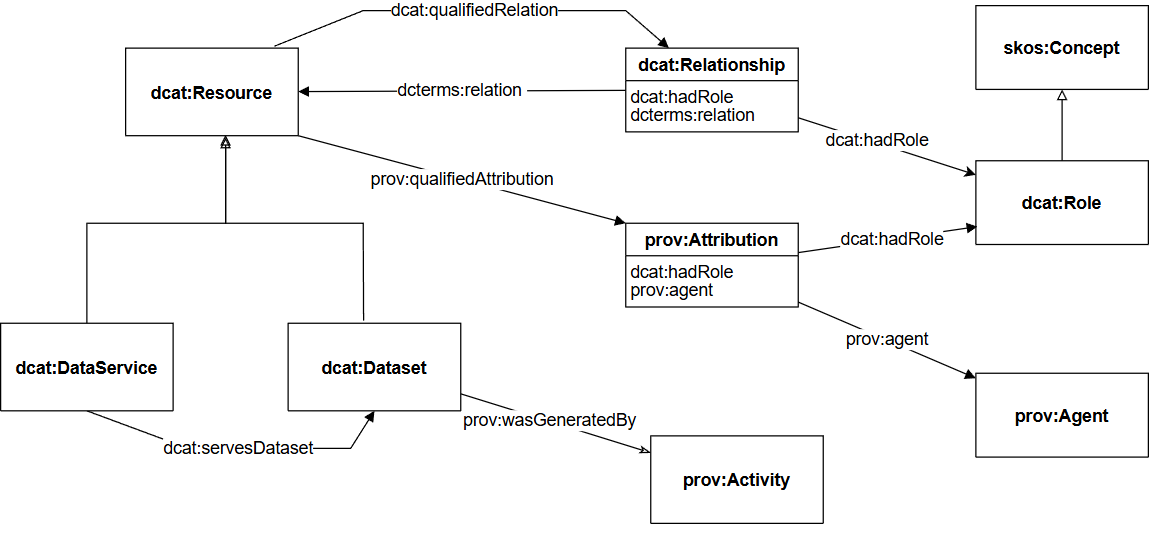
\includegraphics[width=1\textwidth]{figures/dcat.png}
    \caption{DCAT standard - prikazuje osnovne klase i svojstva za opisivanje kataloga podataka~\cite{dcat2020}}
    \label{fig:dcat_standard}
\end{figure}
\chapter{Korištene tehnologije i alati}
\label{ch:technologies}

\selectlanguage{croatian}

Realizacija sustava ovakve složenosti nužno je podrazumijevala selekciju skupa suvremenih i međusobno komplementarnih tehnologija. Ovo poglavlje detaljno obrazlaže izbor svake od ključnih tehnologija, koje su klasificirane u dvije temeljne skupine: tehnologije za upravljanje podacima i komponente umjetne inteligencije. Važno je napomenuti da redoslijed predstavljanja prati logički tok - prvo se opisuju tehnologije za rad s podacima koje čine temelj sustava, a zatim komponente umjetne inteligencije koje omogućavaju njihovu inteligentnu obradu.

\section{Tehnologije za upravljanje podacima}

Ova sekcija opisuje temeljne tehnologije koje omogućuju strukturirano opisivanje, pohranu i dohvat podataka unutar sustava. Predstavljene su redom kojim se koriste u sustavu: prvo SPARQL kao ciljni upitni jezik, zatim DCAT standard koji definira strukturu metapodataka, te naposljetku ChromaDB kao moderna vektorska baza podataka.

\subsection{SPARQL (SPARQL Protocol and RDF Query Language)}

SPARQL predstavlja službeni upitni jezik W3C konzorcija, specificiran za interakciju s podacima pohranjenim u RDF (\textit{Resource Description Framework}) formatu~\cite{sparql2013}. S obzirom na to da EU Portal otvorenih podataka, kao i brojni drugi suvremeni portali, svoje metapodatke izlaže putem javno dostupnog SPARQL \textit{endpoint}-a, kompetentno korištenje ovog jezika nameće se kao imperativ za pristup podacima.

Za razliku od SQL-a, koji operira nad relacijskim tablicama s fiksnom shemom, SPARQL djeluje nad grafom sačinjenim od trojki oblika subjekt-predikat-objekt. Ova fundamentalna razlika omogućava SPARQL-u veću fleksibilnost u radu s heterogenim i distribuiranim podacima. Njegova sintaksa omogućuje formuliranje složenih upita, uključujući:

\begin{itemize}
    \item \textbf{Spajanje podataka} iz različitih dijelova grafa kroz \texttt{JOIN} operacije
    \item \textbf{Višestruko filtriranje} kroz \texttt{FILTER} klauzule s bogatim skupom funkcija
    \item \textbf{Agregacijske funkcije} poput \texttt{COUNT}, \texttt{SUM}, \texttt{AVG} za statističke analize
    \item \textbf{Dohvaćanje opcionalnih podataka} kroz \texttt{OPTIONAL} klauzule
    \item \textbf{Federacijske upite} koji kombiniraju podatke s više različitih \textit{endpoint}-a
\end{itemize}

Primjer jednostavnog SPARQL upita koji dohvaća sve skupove podataka o okolišu:

\begin{lstlisting}[language=SPARQL, caption=Primjer SPARQL upita za dohvaćanje skupova podataka o okolišu]
PREFIX dcat: <http://www.w3.org/ns/dcat#>
PREFIX dct: <http://purl.org/dc/terms/>

SELECT ?dataset ?title ?description
WHERE {
  ?dataset a dcat:Dataset ;
           dct:title ?title ;
           dct:description ?description ;
           dcat:theme <http://publications.europa.eu/resource/authority/data-theme/ENVI> .
}
LIMIT 100
\end{lstlisting}

Ova izražajnost čini SPARQL prikladnim alatom za kompleksne analize, ali istovremeno i kompleksnim za učenje i korištenje. Sintaksa zahtijeva poznavanje RDF modela podataka, razumijevanje \textit{namespace} koncepta te vladanje semantikom različitih tipova obrazaca (\textit{pattern}) pretraživanja. U kontekstu ovog rada, SPARQL je ciljni jezik u koji se vrši prevođenje korisničkih upita s prirodnog jezika, što predstavlja ključni izazov koji sustav rješava.

\subsection{DCAT (Data Catalog Vocabulary)}

DCAT (\textit{Data Catalog Vocabulary}) je RDF rječnik čija je primarna funkcija standardizirano opisivanje kataloga podataka i pripadajućih skupova podataka~\cite{dcat2020}. Razvijen je od strane W3C konzorcija s ciljem omogućavanja interoperabilnosti između različitih portala otvorenih podataka, čime se stvara preduvjet za njihovo federacijsko pretraživanje i integraciju.

DCAT definira hijerarhijsku strukturu metapodataka kroz tri glavne klase:

\begin{enumerate}
    \item \textbf{\texttt{dcat:Catalog}} - predstavlja kolekciju ili katalog skupova podataka
    \item \textbf{\texttt{dcat:Dataset}} - opisuje pojedinačni skup podataka
    \item \textbf{\texttt{dcat:Distribution}} - predstavlja konkretnu distribuciju skupa podataka u određenom formatu
\end{enumerate}

\begin{figure}[htbp]
    \centering
    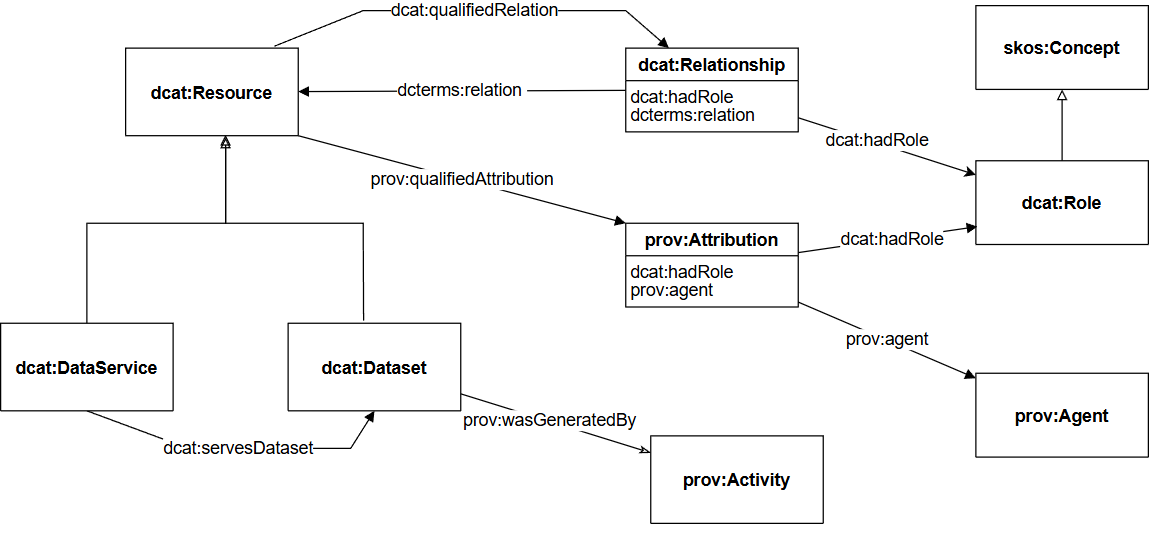
\includegraphics[width=1\textwidth]{figures/dcat.png}
    \caption{DCAT konceptualni model - prikazuje osnovne klase i njihove međusobne veze~\cite{dcat2020}}
    \label{fig:dcat_conceptual_model}
\end{figure}

\subsubsection{DCAT-AP (Application Profile for Data Portals in Europe)}

Za potrebe europskih institucija, razvijen je DCAT-AP (\textit{Application Profile for data portals in Europe}), specifičan profil koji normira upotrebu DCAT rječnika~\cite{dcatap2020}. DCAT-AP definira precizna pravila o tome koje su klase i svojstva:

\begin{itemize}
    \item \textbf{Obavezna (\textit{mandatory})} - moraju biti prisutna za svaki entitet
    \item \textbf{Preporučena (\textit{recommended})} - trebala bi biti prisutna kada su dostupna
    \item \textbf{Opcionalna (\textit{optional})} - mogu biti uključena po potrebi
\end{itemize}

Za klasu \texttt{dcat:Dataset}, DCAT-AP definira sljedeća obavezna svojstva:

\begin{itemize}
    \item \texttt{dct:title} - naslov skupa podataka
    \item \texttt{dct:description} - opis skupa podataka
    \item \texttt{dcat:distribution} - veza na barem jednu distribuciju
\end{itemize}

Preporučena svojstva uključuju:

\begin{itemize}
    \item \texttt{dct:publisher} - organizacija odgovorna za publiciranje
    \item \texttt{dcat:theme} - tematska kategorija iz kontroliranog rječnika
    \item \texttt{dcat:keyword} - ključne riječi za pretraživanje
    \item \texttt{dct:spatial} - geografsko pokrivanje podataka
    \item \texttt{dct:temporal} - vremensko pokrivanje podataka
    \item \texttt{dct:issued} - datum prvog publiciranja
    \item \texttt{dct:modified} - datum zadnje izmjene
\end{itemize}

Poznavanje ove specifikacije od presudne je važnosti za razvijeni sustav. Informacija da svaki skup podataka mora posjedovati određena svojstva pruža ključne smjernice jezičnom modelu pri konstrukciji upita. Također, razumijevanje hijerarhije i međusobnih veza između klasa omogućava generiranje složenijih upita koji navigiraju kroz graf metapodataka.

\begin{figure}[htbp]
    \centering
    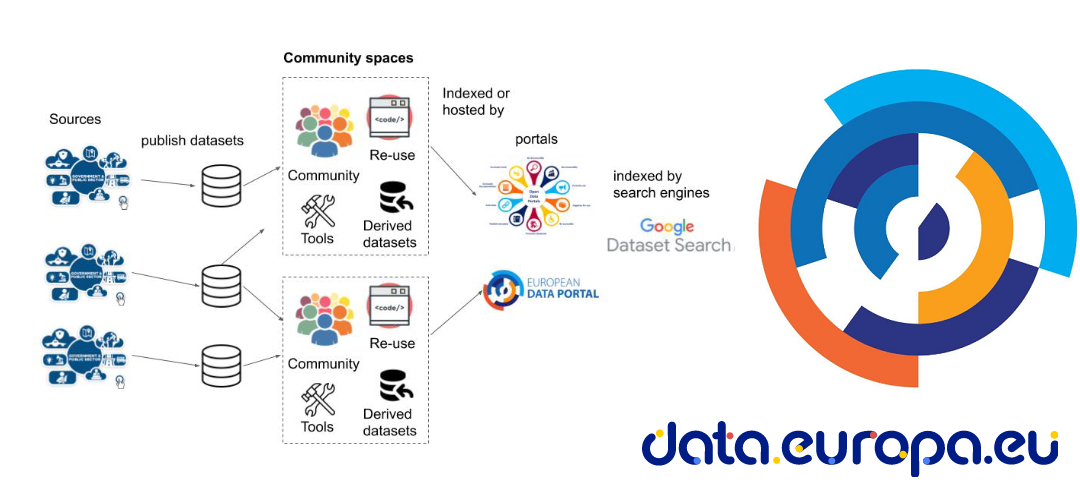
\includegraphics[width=1\textwidth]{figures/Data_Europe.png}
    \caption{EU Portal otvorenih podataka - sučelje koje koristi DCAT standard za organizaciju podataka}
    \label{fig:eu_data_portal}
\end{figure}

\subsection{ChromaDB Vektorska Baza Podataka}

Tradicionalne relacijske i NoSQL baze podataka nisu projektirane za pretragu temeljenu na semantičkoj sličnosti. Njihovi indeksi optimizirani su za egzaktno podudaranje ili pretraživanje po rasponu vrijednosti, ali ne mogu rukovati visokodimenzionalnim vektorskim reprezentacijama. U tu svrhu razvijene su specijalizirane vektorske baze podataka. Za potrebe ovog projekta, odabrana je ChromaDB zbog nekoliko prednosti:

\begin{itemize}
    \item \textbf{Jednostavnost korištenja} - Python sučelje koje ne zahtijeva kompleksnu konfiguraciju
    \item \textbf{Performanse} - optimiziran za brzo pretraživanje kroz velike kolekcije vektora
    \item \textbf{Fleksibilnost} - podrška za različite metrike sličnosti i tipove \textit{embedding} modela
    \item \textbf{\textit{Open source}} licenca - omogućava prilagodbu i proširivanje prema potrebi
    \item \textbf{Integracija s popularnim okvirima} - izravna podrška za LangChain i druge AI alate
\end{itemize}

\begin{figure}[h!]
    \centering
    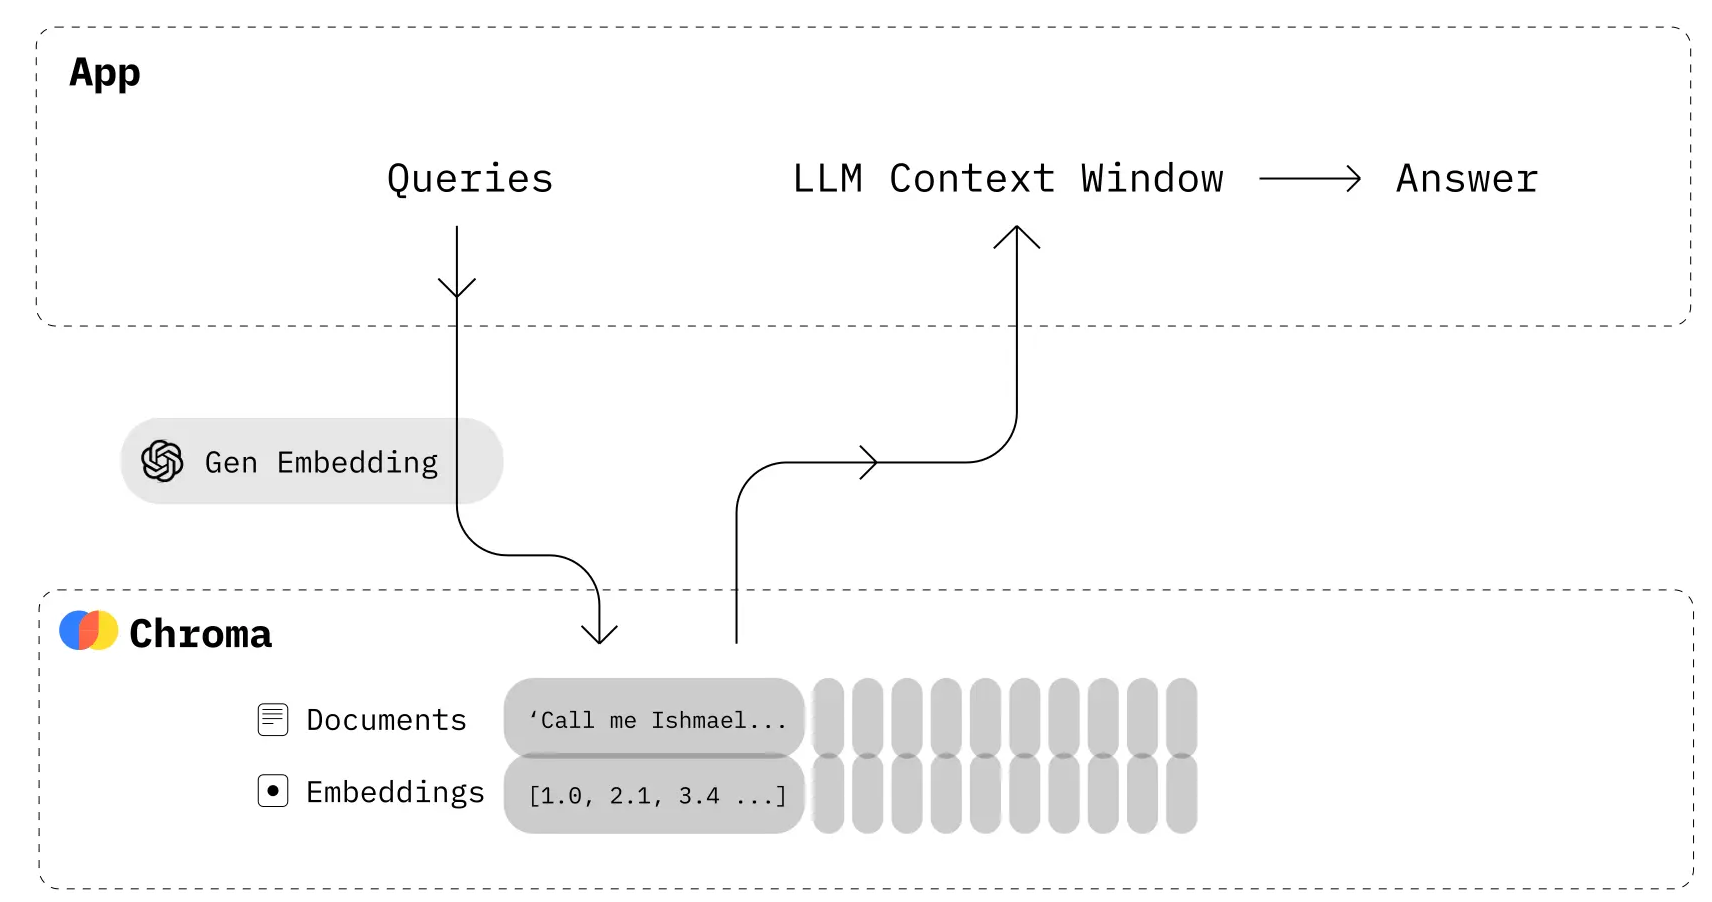
\includegraphics[width=1\textwidth]{figures/chroma.png}
    \caption{ChromaDB arhitektura - prikazuje komponente vektorske baze podataka i tok obrade podataka}
    \label{fig:chromadb_architecture}
\end{figure}

ChromaDB pohranjuje podatke u obliku visokodimenzionalnih numeričkih vektora, poznatih kao ugradbe (\textit{embeddings}), gdje svaki vektor predstavlja sažetu semantičku reprezentaciju određenog tekstualnog fragmenta. Ovi vektori tipično imaju između 384 i 1536 dimenzija, ovisno o korištenom modelu za generiranje \textit{embeddings}-a.

Proces rada s ChromaDB odvija se kroz nekoliko koraka:

\begin{enumerate}
    \item \textbf{Generiranje \textit{embedding}-a} - tekstualni podaci se transformiraju u vektorske reprezentacije
    \item \textbf{Pohrana} - vektori se pohranjuju zajedno s metapodacima u optimiziranu strukturu podataka
    \item \textbf{Indeksiranje} - stvaraju se specijalizirani indeksi za brzo pretraživanje (npr. HNSW - \textit{Hierarchical Navigable Small World})
    \item \textbf{Pretraživanje} - korisnikov upit se također pretvara u vektor te se traže najsličniji vektori u bazi
    \item \textbf{Rangiranje} - rezultati se rangiraju prema stupnju sličnosti (tipično kosinusna sličnost)
\end{enumerate}

U arhitekturi ovog sustava, ChromaDB se koristi za pohranu:

\begin{itemize}
    \item \textbf{Parova pitanje-SPARQL upit} - omogućava pronalaženje sličnih upita iz prošlosti
    \item \textbf{Fragmenata DCAT sheme} - pomaže u kontekstualizaciji korisničkih upita
    \item \textbf{Opisa klasa i svojstava} - pruža semantički kontekst za generiranje upita
    \item \textbf{Primjera uspješnih upita} - služe kao predlošci za nove upite
\end{itemize}

Izbor kosinusne sličnosti kao primarne metrike zaslužuje dodatno objašnjenje. Iako postoje alternative poput euklidske udaljenosti ili Manhattan udaljenosti, kosinusna sličnost pokazala se prikladnom za semantičko pretraživanje iz nekoliko razloga:

\begin{itemize}
    \item Mjeri orijentaciju vektora u prostoru, što bolje odražava semantičku sličnost
    \item Nije osjetljiva na magnitudu vektora, što je važno za tekstove različite duljine
    \item Vrijednosti su normalizirane između -1 i 1, što olakšava interpretaciju
    \item Računski je jednostavnija od kompleksnijih hibridnih metoda
\end{itemize}

Pitanje zašto ne koristiti hibridne pristupe koji kombiniraju vektorsko pretraživanje s tradicionalnim "\textit{bag of words}" metodama je opravdano. Takvi pristupi mogu pružiti dodatne prednosti, posebno za specifične domene. Međutim, za potrebe ovog prototipa, čista vektorska pretraga pokazala se dostatnom iz sljedećih razloga:

\begin{itemize}
    \item Jednostavnost implementacije i održavanja
    \item Konzistentnost rezultata kroz različite tipove upita
    \item Dovoljna preciznost za identificirane slučajeve korištenja
    \item Mogućnost naknadnog proširenja s hibridnim pristupom
\end{itemize}

\section{Komponente umjetne inteligencije}

Ova sekcija opisuje komponente umjetne inteligencije koje sustavu daju sposobnost razumijevanja, rezoniranja i generiranja prirodnog i formalnog jezika. Redoslijed predstavljanja slijedi logiku njihove uporabe u sustavu: od jezičnih modela koji generiraju upite, preko modela za stvaranje semantičkih reprezentacija, do orkestracijskih okvira koji sve povezuju.

\subsection{Veliki jezični modeli (LLM) - OpenAI GPT-4}

Veliki jezični modeli (\textit{Large Language Models} - LLM) predstavljaju razvojni napredak u području obrade prirodnog jezika. Ovi modeli, trenirani na velikim količinama tekstualnih podataka, pokazuju sposobnosti razumijevanja konteksta, rezoniranja i generiranja koherentnog teksta. U sklopu ovog rada, korišten je OpenAI-jev model GPT-4~\cite{openai2023gpt4}.

GPT-4 odabran je zbog nekoliko karakteristika:

\begin{itemize}
    \item \textbf{Sposobnosti razumijevanja} - može interpretirati složene instrukcije i kontekst
    \item \textbf{Generiranje strukturiranog koda} - sposobnost stvaranja sintaksno ispravnog SPARQL koda
    \item \textbf{Kontekstualno rezoniranje} - razumijevanje veza između različitih koncepata u upitu
    \item \textbf{Višejezičnost} - rad s upitima na hrvatskom i engleskom jeziku
    \item \textbf{Stabilnost i pouzdanost} - konzistentnost u generiranju odgovora
\end{itemize}

U kontekstu ovog sustava, GPT-4 se primjenjuje u \textit{Generation} fazi RAG procesa. Njegov zadatak uključuje:

\begin{enumerate}
    \item \textbf{Analizu korisničkog upita} - razumijevanje namjere i identificiranje ključnih entiteta
    \item \textbf{Sinteza kontekstualnih informacija} - kombiniranje korisničkog upita s dohvaćenim primjerima i shemom
    \item \textbf{Generiranje SPARQL koda} - prevođenje prirodnog jezika u formalni upitni jezik
    \item \textbf{Validacija logike} - osiguravanje da generirani upit odgovara korisničkoj namjeri
\end{enumerate}

Važno je napomenuti ograničenja GPT-4 modela koja utječu na dizajn sustava:

\begin{itemize}
    \item \textbf{Ograničenje konteksta} - maksimalno 8,000 tokena za standardnu verziju
    \item \textbf{Stohastička priroda} - može generirati različite odgovore za isti upit
    \item \textbf{Nedostatak stvarnog znanja o specifičnoj shemi} - zahtijeva eksplicitno pružanje konteksta
    \item \textbf{Troškovi API poziva} - mogu biti značajni za intenzivnu upotrebu
    \item \textbf{Latencija} - vrijeme odziva može biti nekoliko sekundi
\end{itemize}

Ova ograničenja motivirala su uporabu RAG arhitekture koja minimizira broj poziva prema modelu i maksimizira kvalitetu konteksta koji mu se pruža.

\subsection{Modeli za semantičke ugradbe - Sentence Transformers}

Da bi se tekstualni podaci mogli pretraživati po semantičkoj sličnosti, nužno ih je prethodno preslikati u numerički, vektorski prostor. Taj proces, poznat kao generiranje ugradbi (\textit{embedding generation}), temeljna je komponenta sustava za pretraživanje i analizu teksta.

Za potrebe ovog rada korištena je biblioteka \textit{Sentence Transformers}~\cite{reimers2019sentence}, koja omogućava generiranje semantičkih reprezentacija rečenica i paragrafa. Specifično je korišten model \texttt{all-MiniLM-L6-v2}, koji je odabran nakon testiranja nekoliko alternativa.

Karakteristike modela \texttt{all-MiniLM-L6-v2}:

\begin{itemize}
    \item \textbf{Dimenzionalnost} - generira 384-dimenzijske vektore
    \item \textbf{Brzina} - može procesirati ~14,000 rečenica po sekundi na modernom CPU-u
    \item \textbf{Veličina} - samo 80MB, što omogućava brzo učitavanje i malu memorijsku potrošnju
    \item \textbf{Kvaliteta} - dobre rezultate na standardnim \textit{benchmark} testovima
    \item \textbf{Višejezičnost} - funkcionira s hrvatskim i engleskim tekstom
\end{itemize}

Proces generiranja \textit{embeddings}-a odvija se kroz nekoliko faza:

\begin{enumerate}
    \item \textbf{Tokenizacija} - tekst se dijeli na osnovne jedinice (tokene)
    \item \textbf{Enkodiranje} - tokeni se procesiraju kroz transformer arhitekturu
    \item \textbf{Agregacija} - reprezentacije tokena se kombiniraju u jedinstveni vektor
    \item \textbf{Normalizacija} - vektor se normalizira za lakše računanje sličnosti
\end{enumerate}

U kontekstu ovog sustava, \textit{Sentence Transformers} se koriste za:

\begin{itemize}
    \item Generiranje \textit{embeddings}-a za korisničke upite
    \item Stvaranje vektorskih reprezentacija primjera u bazi
    \item Enkodiranje fragmenata DCAT sheme
    \item Omogućavanje brzog semantičkog pretraživanja
\end{itemize}

Kvaliteta \textit{embeddings}-a direktno utječe na uspješnost RAG sustava. Bolji \textit{embeddings} znače precizniji dohvat relevantnih primjera, što rezultira kvalitetnijim kontekstom za jezični model i, konačno, boljim SPARQL upitima.

\subsection{Orkestracijski okviri - LangChain}

Razvoj kompleksnih aplikacija temeljenih na velikim jezičnim modelima često podrazumijeva orkestraciju višestrukih komponenti u koherentan procesni lanac. Potrebno je koordinirati dohvat podataka, njihovu obradu, pozive prema različitim modelima, parsiranje odgovora i rukovanje greškama. LangChain~\cite{chase2022langchain} je softverski okvir koji pojednostavljuje ovaj proces kroz visoku razinu apstrakcije.

LangChain nudi nekoliko ključnih koncepata:

\begin{itemize}
    \item \textbf{Lanci (\textit{Chains})} - sekvencijalno povezivanje operacija
    \item \textbf{Agenti (\textit{Agents})} - autonomni sustavi koji mogu donositi odluke
    \item \textbf{Alati (\textit{Tools})} - funkcionalnosti koje agenti mogu koristiti
    \item \textbf{Memorija (\textit{Memory})} - održavanje konteksta kroz interakcije
    \item \textbf{Promptovi} - strukturirani predlošci za komunikaciju s modelima
\end{itemize}

U ovom radu, LangChain se koristi za dvije ključne svrhe:

\subsubsection{Orkestracija RAG pipeline-a}

LangChain omogućava elegantno povezivanje pojedinačnih koraka RAG procesa:

\begin{enumerate}
    \item Dohvat relevantnih primjera iz ChromaDB baze
    \item Dohvat informacija o DCAT shemi
    \item Dinamička konstrukcija prompta s kontekstom
    \item Poziv GPT-4 modela s optimiziranim parametrima
    \item Parsiranje i validacija generiranog SPARQL koda
    \item Rukovanje greškama i pokušaji ponovnog generiranja
\end{enumerate}

\subsubsection{Upravljanje multimodalnim agentom}

LangChain-ov agentski okvir omogućava stvaranje inteligentnog asistenta koji može:

\begin{itemize}
    \item Analizirati korisnički upit i identificirati strategiju
    \item Autonomno odlučiti koje alate koristiti (SPARQL, REST API, similarity search)
    \item Paralelno izvršavati različite strategije pretraživanja
    \item Inteligentno kombinirati rezultate iz različitih izvora
    \item Prilagoditi pristup na temelju dobivenih rezultata
\end{itemize}

Prednosti korištenja LangChain-a uključuju:

\begin{itemize}
    \item \textbf{Modularnost} - lako dodavanje novih komponenti
    \item \textbf{Standardizacija} - konzistentan način rada s različitim modelima
    \item \textbf{Skalabilnost} - podrška za asinkrono izvršavanje
    \item \textbf{Ekstenzibilnost} - mogućnost stvaranja prilagođenih komponenti
    \item \textbf{Debugging} - ugrađeni alati za praćenje i analizu
\end{itemize}

\chapter{Arhitektura sustava}
\label{ch:system_architecture}

Uspješna implementacija složenog softverskog rješenja uvjetovana je postojanjem dobro definirane arhitekture. Ovo poglavlje pruža detaljan opis arhitekture razvijenog sustava, koristeći standardiziranu UML notaciju za vizualizaciju komponenti, njihovih međuodnosa i cjelokupnog toka podataka. Arhitektura je dizajnirana s naglaskom na modularnost, skalabilnost i održivost, omogućavajući lakše proširivanje i prilagodbu budućim zahtjevima.

\section{Korištene tehnologije}

Ključne tehnologije korištene u implementaciji uključuju ChromaDB kao vektorsku bazu podataka za pohranu i pretraživanje semantičkih ugradbi, Sentence Transformers modele za generiranje vektorskih reprezentacija teksta, i OpenAI GPT-4 model za generiranje SPARQL upita iz prirodnog jezika.

LangChain okvir korišten je za orkestraciju različitih komponenti sustava i upravljanje agentima koji omogućavaju složene zadatke poput multimodalnog pretraživanja i inteligentne sinteze rezultata. Ova arhitektura omogućava modularnost i proširivost sustava.

\section{Ključne funkcionalnosti}

Automatska ekstrakcija sheme iz SPARQL endpointa omogućava dinamičko prilagođavanje sustava promjenama u strukturi podataka. Ova funkcionalnost je ključna za održavanje točnosti generiranih upita i omogućava sustavu da radi s različitim portalima otvorenih podataka.

\begin{figure}[htbp]
    \centering
    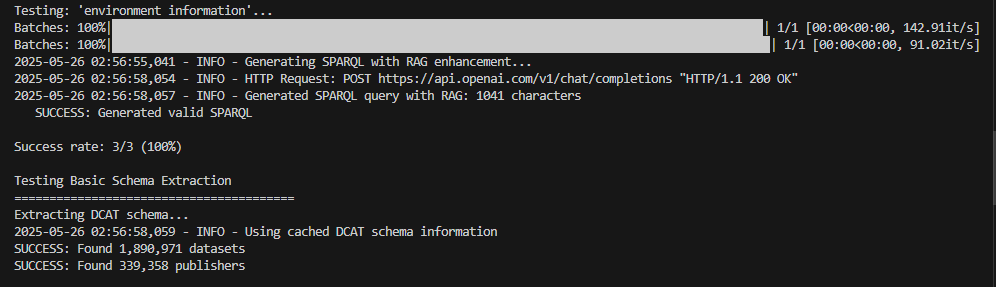
\includegraphics[width=1\textwidth]{figures/izvjestaj_image_11.png}
    \caption{Ekstrakcija sheme i validacija generiranog SPARQL upita}
    \label{fig:schema_extraction}
\end{figure}

Validacija upita implementirana je kroz dvostupanjski proces koji uključuje sintaksnu i semantičku provjeru. Ovo osigurava da se ne izvršavaju neispravni upiti koji mogu uzrokovati probleme s performansama ili pogrešne rezultate.

Multimodalni pristup pretraživanju omogućava kombiniranje različitih strategija za sveobuhvatno otkrivanje skupova podataka. Ovo uključuje RAG-prošireno SPARQL pretraživanje, REST API pozive i pronalaženje sličnih skupova podataka.

\begin{figure}[htbp]
    \centering
    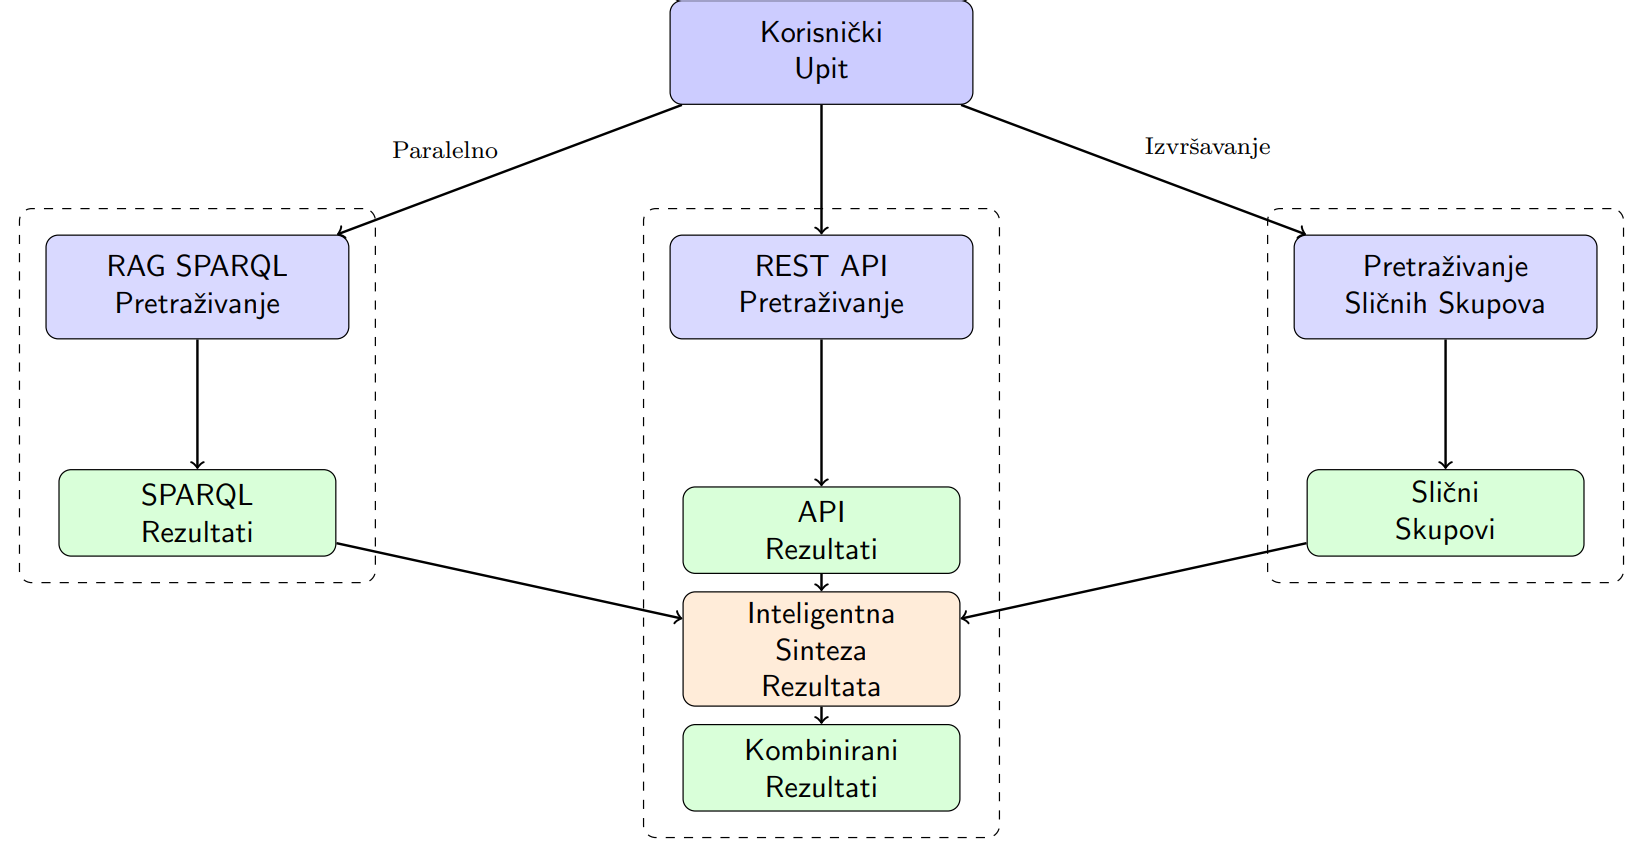
\includegraphics[width=1\textwidth]{figures/multimodal_search.png}
    \caption{Multimodalno pretraživanje - prikazuje različite strategije i njihovu integraciju}
    \label{fig:multimodal_search}
\end{figure}

\section{Arhitektura i skalabilnost}

Sustav je dizajniran da bude skalabilan i održiv, s jasno definiranim sučeljima između komponenti i mehanizmima rukovanja greškama. Ova arhitektura omogućava lako proširivanje i prilagodbu drugim portalima otvorenih podataka.

\begin{figure}[htbp]
    \centering
    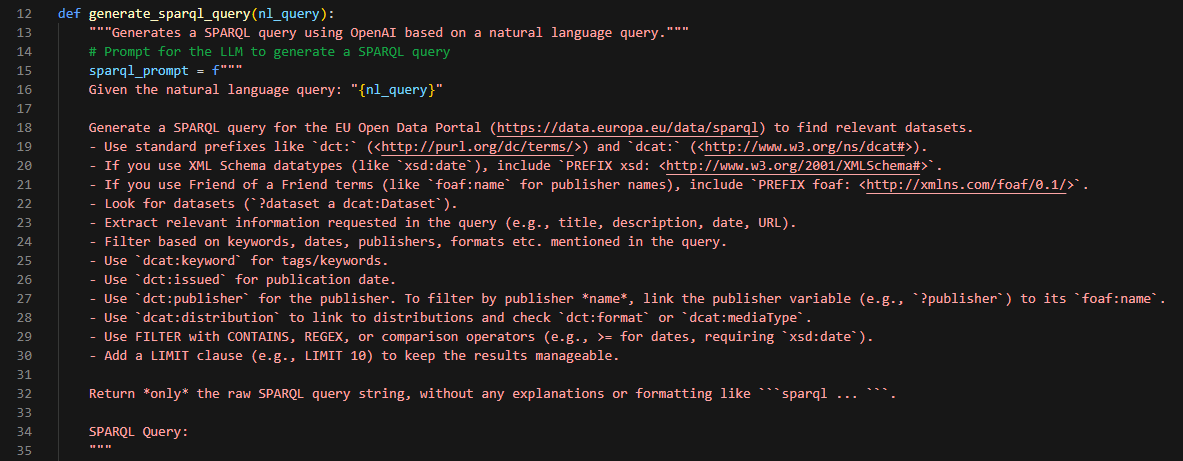
\includegraphics[width=1\textwidth]{figures/izvjestaj_image_13.png}
    \caption{Skalabilnost sustava - prikazuje mogućnosti proširivanja i optimizacije}
    \label{fig:system_scalability}
\end{figure}

Sustav pruža sučelje koje omogućava pristup kompleksnim skupovima podataka kroz prirodni jezik. Ovo demokratizira pristup otvorenim podacima i omogućava širu primjenu u različitim domenama.

\begin{figure}[htbp]
    \centering
    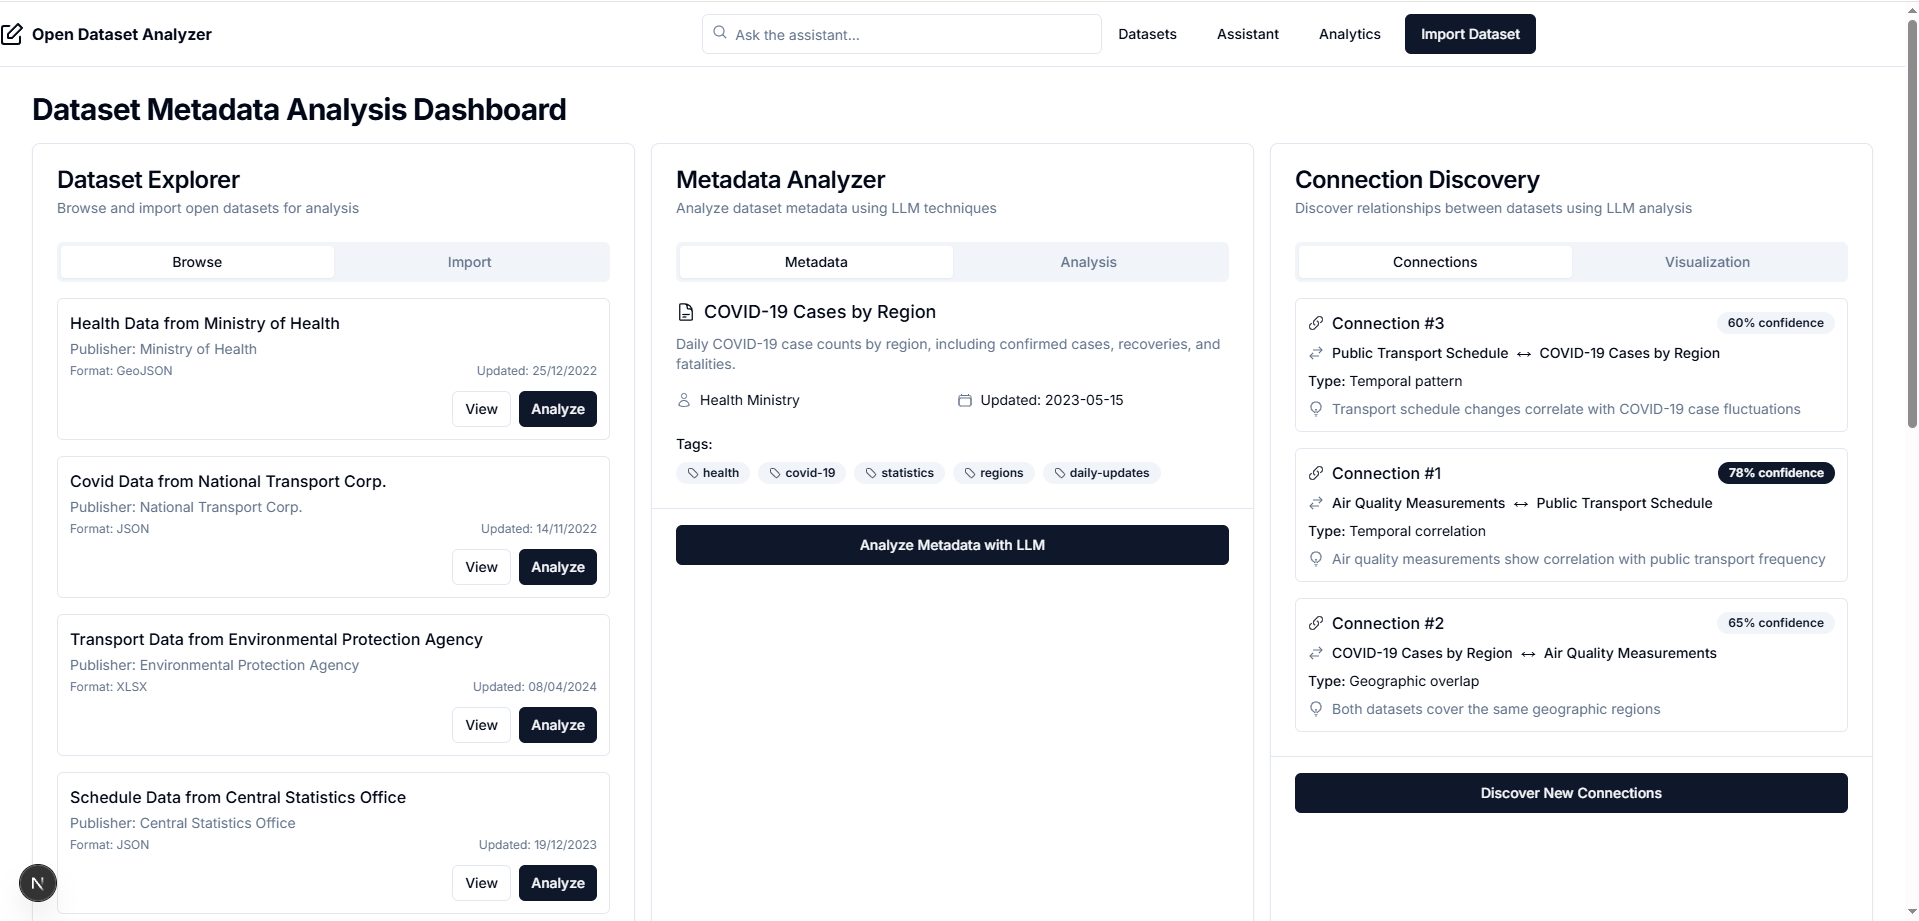
\includegraphics[width=1\textwidth]{figures/izvjestaj_image_4.png}
    \caption{Sučelje sustava - prikazuje dizajn i funkcionalnosti}
    \label{fig:user_interface}
\end{figure}

Sustav je dizajniran kao modularna arhitektura s jasno definiranim sučeljima između komponenti. Glavni razlog za ovakav pristup je mogućnost nezavisnog razvoja i testiranja pojedinačnih dijelova, što se pokazalo ključnim tijekom implementacije kada je bilo potrebno ispravljati probleme s vektorskim pretraživanjem ili optimizirati LLM pozive.

Arhitektura se sastoji od tri glavna sloja. Sloj pohrane koristi ChromaDB~\cite{wang2023vector} kao vektorsku bazu podataka, Sentence Transformers modele~\cite{reimers2019sentence} za generiranje vektorskih reprezentacija, i OpenAI GPT-4 model~\cite{brown2020language} za generiranje SPARQL upita. ChromaDB omogućava brzo pretraživanje sličnosti i podržava pohranu meta podataka.

Sloj obrade uključuje Sentence Transformers model all-MiniLM-L6-v2 za generiranje embeddinga. Ovaj model je odabran nakon testiranja nekoliko alternativa - pokazao se kao adekvatan balans između kvalitete embeddinga, brzine generiranja i veličine modela. Model generira 384-dimenzijske vektore što je dovoljno za hvatanje semantičkih razlika.

LangChain okvir~\cite{liu2023survey} korišten je za orkestraciju različitih komponenti sustava i upravljanje agentima koji omogućavaju složene zadatke poput multimodalnog pretraživanja i inteligentne sinteze rezultata.

OpenAI GPT-4 je korišten za generiranje SPARQL upita. Model pokazuje dobre rezultate kada ima dovoljno kontekstualnih informacija, ali ima ograničenja s tokenima što može biti problematično za složene upite. Također, troškovi API poziva mogu biti značajni za intenzivnu upotrebu.

\begin{figure}[htbp]
    \centering
    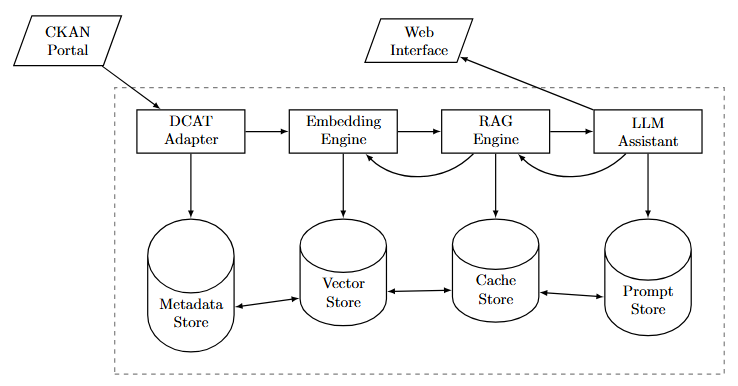
\includegraphics[width=1\textwidth]{figures/system_architecture.png}
    \caption{Arhitektura sustava - prikazuje tok podataka kroz različite komponente}
    \label{fig:system_architecture}
\end{figure}

\section{Implementacija RAG sustava i vektorske baze}

RAG sustav~\cite{lewis2020retrieval} je implementiran u src/rag\_system.py i predstavlja srce cijelog sustava. Glavna klasa RAGSystem upravlja svim aspektima RAG pipeline-a od generiranja embeddinga do izvršavanja upita.

Inicijalizacija sustava uključuje postavljanje ChromaDB klijenta, učitavanje Sentence Transformers modela i konfiguraciju OpenAI klijenta. ChromaDB koristi trajno pohranjivanje što omogućava da se embeddingi sačuvaju između pokretanja sustava. Ovo je bilo ključno za performanse jer generiranje embeddinga može biti sporo, posebno za velike kolekcije teksta.

Generiranje embeddinga se vrši kroz metodu generate\_embedding koja koristi Sentence Transformers model. Implementacija uključuje caching mehanizam koji sprečava ponovno generiranje embeddinga za iste tekstove. Caching je implementiran kao jednostavan dictionary u memoriji, ali za produkcijsku upotrebu bi trebao biti implementiran kao Redis ili sličan sustav.

Dodavanje primjera upita u vektorsku bazu se vrši kroz metodu add\_query\_example. Svaki primjer se sastoji od pitanja na prirodnom jeziku, odgovarajućeg SPARQL upita, opisa i tagova. Embedding se generira za pitanje, a metadata se sprema zajedno s embeddingom. Ovo omogućava kasnije pretraživanje sličnih primjera na temelju semantičke sličnosti.

\begin{lstlisting}[language=Python, caption=Implementacija dodavanja primjera u vektorsku bazu]
def add_query_example(self, example: QueryExample) -> str:
    """Dodaj primjer pitanje-upit par u vektorsku bazu"""
    
    # Provjeri cache za embedding
    cache_key = f"embedding_{hash(example.question)}"
    if cache_key in self.embedding_cache:
        embedding = self.embedding_cache[cache_key]
    else:
        embedding = self._generate_embedding(example.question)
        self.embedding_cache[cache_key] = embedding
    
    # Generiraj jedinstveni ID
    doc_id = f"example_{len(self.query_examples_collection.get()['ids'])}"
    
    # Spremi u ChromaDB
    self.query_examples_collection.add(
        documents=[example.question],
        embeddings=[embedding],
        metadatas=[{
            "sparql_query": example.sparql_query,
            "endpoint": example.endpoint,
            "description": example.description,
            "tags": json.dumps(example.tags),
            "added_at": datetime.now().isoformat(),
            "success_rate": example.success_rate if hasattr(example, 'success_rate') else None
        }],
        ids=[doc_id]
    )
    
    return doc_id
\end{lstlisting}

Semantička pretraga sličnih primjera je implementirana kroz metodu retrieve\_similar\_examples. Metoda koristi kosinusnu sličnost za pronalaženje najsličnijih primjera u vektorskom prostoru. Implementacija uključuje opciju za filtriranje rezultata na temelju tagova ili endpointa, što može biti korisno za specifične domene.

\begin{lstlisting}[language=Python, caption=Implementacija semantičke pretrage]
def retrieve_similar_examples(self, query: str, n_results: int = 5, filters: Dict = None) -> List[Dict[str, Any]]:
    """Dohvati slične primjere koristeći vektorsku pretragu"""
    
    # Generiraj ugradbu za upit
    query_embedding = self._generate_embedding(query)
    
    # Postavi filtere ako su zadani
    where_clause = None
    if filters:
        where_clause = {}
        if 'tags' in filters:
            where_clause['tags'] = {'$contains': filters['tags']}
        if 'endpoint' in filters:
            where_clause['endpoint'] = filters['endpoint']
    
    # Izvedi vektorsku pretragu
    results = self.query_examples_collection.query(
        query_embeddings=[query_embedding],
        n_results=n_results,
        where=where_clause
    )
    
    # Obradi rezultate
    similar_examples = []
    if results['documents'] and results['documents'][0]:
        for i, doc in enumerate(results['documents'][0]):
            metadata = results['metadatas'][0][i]
            similar_examples.append({
                "question": doc,
                "sparql_query": metadata.get("sparql_query"),
                "distance": results['distances'][0][i],
                "success_rate": metadata.get("success_rate"),
                "tags": json.loads(metadata.get("tags", "[]"))
            })
    
    return similar_examples
\end{lstlisting}

\begin{figure}[h!]
    \centering
    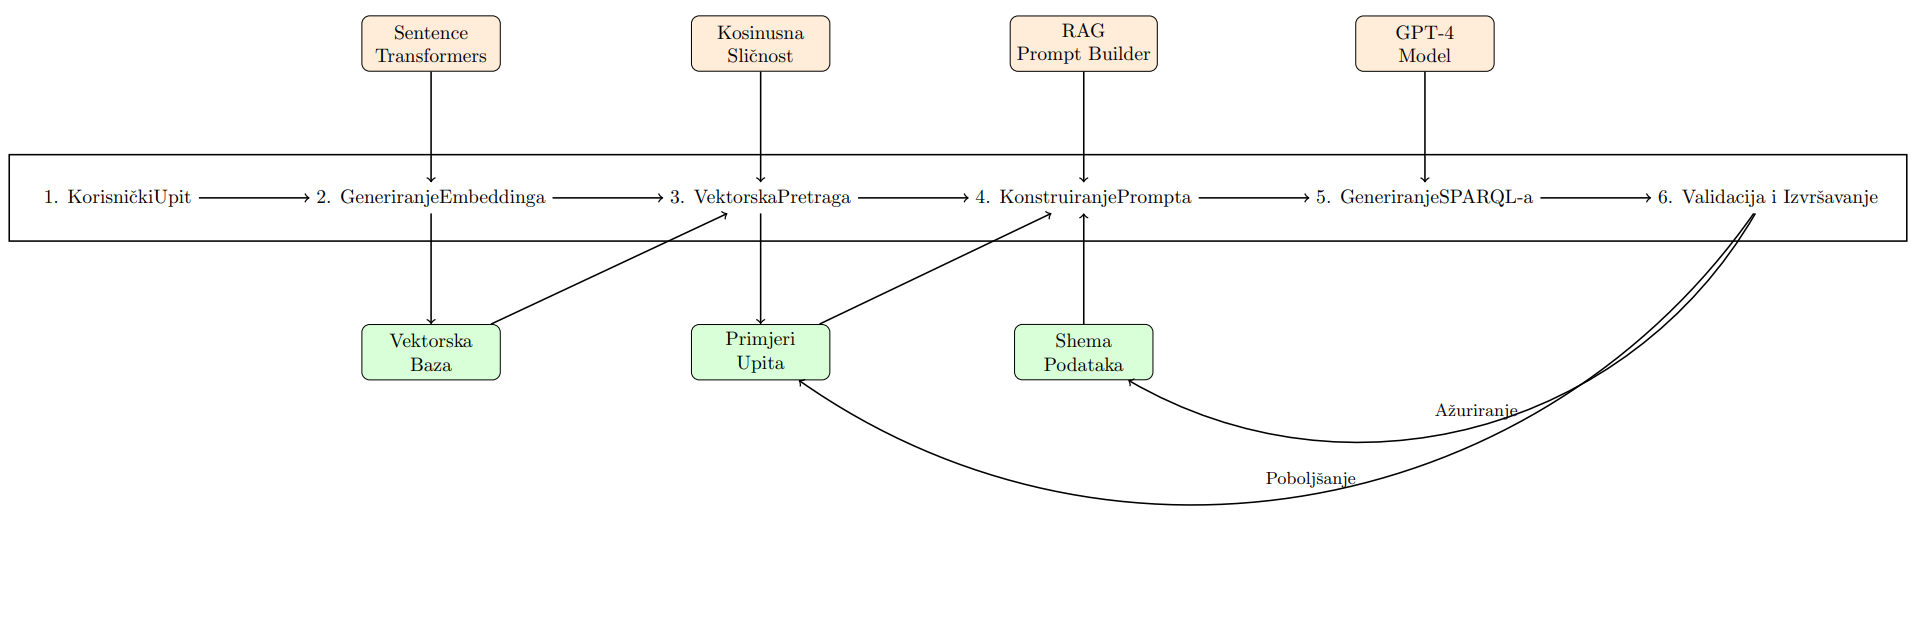
\includegraphics[width=1\textwidth]{figures/rag_pipeline.png}
    \caption{RAG pipeline - prikazuje tok od upita do generiranog SPARQL-a}
    \label{fig:rag_pipeline}
\end{figure}

\section{Generiranje SPARQL upita i prompt engineering}

Generiranje SPARQL upita iz prirodnog jezika je najsloženiji dio sustava. Implementacija koristi RAG pristup gdje se korisnički upit proširuje s relevantnim primjerima i informacijama o shemi prije slanja LLM-u.

Konstruiranje prompta se vrši kroz metodu build\_rag\_prompt koja kombinira korisnički upit s dohvaćenim primjerima i informacijama o shemi. Prompt je strukturiran u nekoliko sekcija: kontekst upita, slični primjeri, informacije o shemi i instrukcije za generiranje. Ova struktura se pokazala kao ključna za kvalitetu generiranih upita.

\begin{lstlisting}[language=Python, caption=Implementacija konstruiranja RAG prompta]
def build_rag_prompt(self, user_query: str, context: str = "") -> str:
    """Konstruiraj poboljšani prompt koristeći RAG tehnologiju"""
    
    # Dohvati slične primjere i informacije o shemi
    similar_examples = self.retrieve_similar_examples(user_query, n_results=3)
    schema_info = self.retrieve_relevant_schema(user_query, n_results=2)
    
    # Počni s osnovnim promptom
    prompt = f"""You are an expert SPARQL query generator for the EU Open Data Portal.
    
User Query: "{user_query}"
{f"Additional Context: {context}" if context else ""}

Your task is to generate a valid SPARQL query that retrieves the requested data.
Use the following examples and schema information as guidance.

## Similar Query Examples:
"""
    
    # Dodaj slične primjere
    for i, example in enumerate(similar_examples):
        prompt += f"""
Example {i+1}:
Question: {example['question']}
SPARQL Query:
{example['sparql_query']}
Distance: {example['distance']:.3f}
"""
    
    # Dodaj informacije o shemi
    if schema_info:
        prompt += "\n## Available Schema Information:\n"
        for i, schema in enumerate(schema_info):
            prompt += f"""
Schema {i+1}:
Classes: {', '.join([cls.get('name', '') for cls in schema['classes'][:10]])}
Properties: {', '.join([prop.get('name', '') for prop in schema['properties'][:15]])}
"""
    
    # Dodaj instrukcije
    prompt += """
## Instructions:
1. Generate a valid SPARQL query that matches the user's intent
2. Use appropriate prefixes (dcat:, dct:, foaf:, etc.)
3. Include proper WHERE clauses and OPTIONAL patterns where needed
4. Limit results to reasonable number (e.g., LIMIT 100)
5. Return only the SPARQL query, no explanations

SPARQL Query:
"""
    
    return prompt
\end{lstlisting}

Generiranje upita se vrši kroz metodu generate\_sparql\_query koja koristi OpenAI GPT-4 model. Implementacija uključuje error handling i retry logiku za slučaj API grešaka. Također, implementiran je mehanizam za validaciju generiranih upita prije izvršavanja.

\begin{lstlisting}[language=Python, caption=Implementacija generiranja SPARQL upita]
def generate_sparql_query(self, user_query: str, context: str = "") -> Dict[str, Any]:
    """Generiraj SPARQL upit iz prirodnog jezika"""
    
    try:
        # Konstruiraj prompt
        prompt = self.build_rag_prompt(user_query, context)
        
        # Pozovi LLM
        response = self.llm.invoke(prompt)
        
        # Ekstraktiraj SPARQL upit iz odgovora
        sparql_query = self._extract_sparql_from_response(response.content)
        
        # Validiraj upit
        validation_result = self.validate_sparql_query(sparql_query)
        
        return {
            "sparql_query": sparql_query,
            "is_valid": validation_result["is_valid"],
            "errors": validation_result.get("errors", []),
            "warnings": validation_result.get("warnings", []),
            "prompt_used": prompt,
            "model_response": response.content
        }
        
    except Exception as e:
        return {
            "sparql_query": None,
            "is_valid": False,
            "errors": [str(e)],
            "prompt_used": prompt if 'prompt' in locals() else None
        }
\end{lstlisting}

\begin{figure}[htbp]
    \centering
    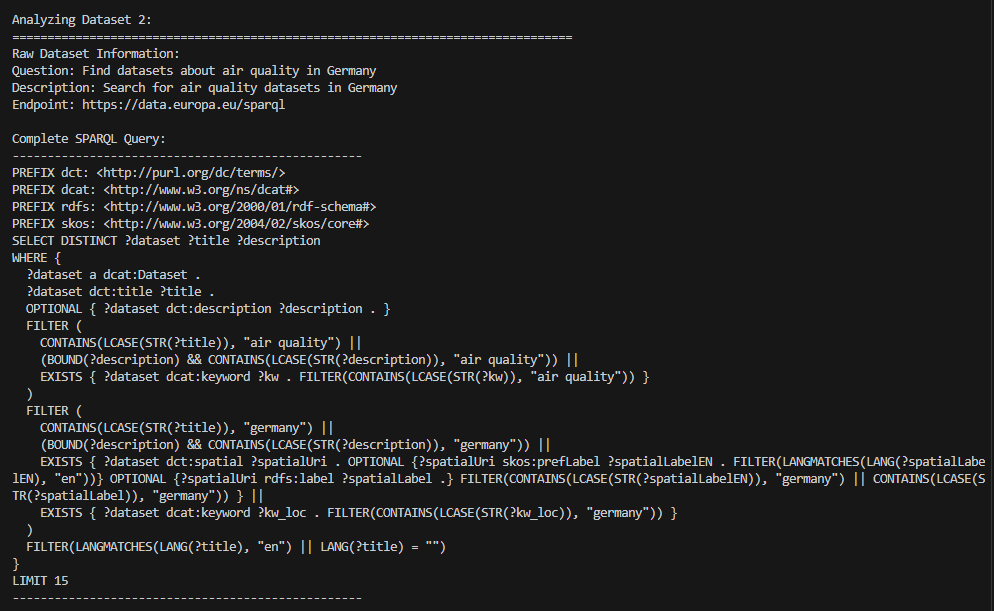
\includegraphics[width=1\textwidth]{figures/izvjestaj_image_53.png}
    \caption{Generiranje SPARQL upita}
    \label{fig:unified_data_assistant}
\end{figure}

Validacija upita je implementirana kroz dvostupanjski proces. Prvi korak je sintaksna validacija kroz SPARQL parser, a drugi korak je testiranje izvršavanja s ograničenim brojem rezultata. Ovo sprečava izvršavanje neispravnih upita koji mogu uzrokovati probleme s performansama.

\begin{figure}[htbp]
    \centering
    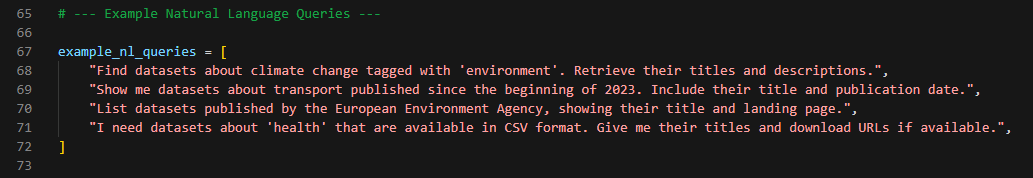
\includegraphics[width=1\textwidth]{figures/izvjestaj_image_84.png}
    \caption{Primjer prompta - struktura i elementi prompta za LLM}
    \label{fig:prompt_example}
\end{figure}

\section{Ekstrakcija sheme i DCAT analiza}

Automatska ekstrakcija sheme iz SPARQL endpointa je ključna komponenta sustava koja omogućava dinamičko prilagođavanje promjenama u strukturi podataka. Implementacija je specifično prilagođena za EU Portal otvorenih podataka i DCAT metapodatke.

VoID deskriptor ekstrakcija se vrši kroz SPARQL upite koji dohvaćaju informacije o strukturi grafa znanja. Implementacija uključuje dohvaćanje broja trojki, različitih subjekata, klasa i svojstava. Ove informacije su ključne za razumijevanje strukture podataka i optimizaciju upita.

\begin{lstlisting}[language=Python, caption=Implementacija VoID deskriptor ekstrakcije]
def get_void_description(self) -> Dict[str, Any]:
    """Ekstraktiraj VoID opis grafa znanja"""
    
    void_query = """
    PREFIX void: <http://rdfs.org/ns/void#>
    PREFIX dct: <http://purl.org/dc/terms/>
    PREFIX foaf: <http://xmlns.com/foaf/0.1/>
    
    SELECT DISTINCT ?dataset ?title ?description ?subjects ?triples ?classes ?properties
    WHERE {
      ?dataset a void:Dataset .
      OPTIONAL { ?dataset dct:title ?title . }
      OPTIONAL { ?dataset dct:description ?description . }
      OPTIONAL { ?dataset void:distinctSubjects ?subjects . }
      OPTIONAL { ?dataset void:triples ?triples . }
      OPTIONAL { ?dataset void:classes ?classes . }
      OPTIONAL { ?dataset void:properties ?properties . }
    }
    LIMIT 10
    """
    
    try:
        results = self._execute_sparql_query(void_query)
        return self._process_void_results(results)
    except Exception as e:
        logger.error(f"Error extracting VoID description: {e}")
        return {}
\end{lstlisting}

DCAT analiza se fokusira na specifične aspekte EU Portala otvorenih podataka. Implementacija dohvaća informacije o skupovima podataka, distribucijama, izdavačima, temama i formatima. Ove informacije omogućavaju generiranje upita koji su optimizirani za specifične karakteristike EU Portala.

\begin{lstlisting}[language=Python, caption=Implementacija DCAT analize]
def analyze_dcat_structure(self) -> Dict[str, Any]:
    """Analiziraj DCAT strukturu grafa znanja"""
    
    dcat_queries = {
        "datasets": """
        PREFIX dcat: <http://www.w3.org/ns/dcat#>
        PREFIX dct: <http://purl.org/dc/terms/>
        
        SELECT ?dataset ?title ?publisher ?theme ?keyword
        WHERE {
          ?dataset a dcat:Dataset .
          OPTIONAL { ?dataset dct:title ?title . }
          OPTIONAL { ?dataset dct:publisher ?publisher . }
          OPTIONAL { ?dataset dcat:theme ?theme . }
          OPTIONAL { ?dataset dcat:keyword ?keyword . }
        }
        LIMIT 100
        """,
        
        "distributions": """
        PREFIX dcat: <http://www.w3.org/ns/dcat#>
        PREFIX dct: <http://purl.org/dc/terms/>
        
        SELECT ?dataset ?distribution ?format ?accessURL
        WHERE {
          ?dataset a dcat:Dataset .
          ?dataset dcat:distribution ?distribution .
          OPTIONAL { ?distribution dcat:mediaType ?format . }
          OPTIONAL { ?distribution dcat:accessURL ?accessURL . }
        }
        LIMIT 100
        """
    }
    
    results = {}
    for query_name, query in dcat_queries.items():
        try:
            results[query_name] = self._execute_sparql_query(query)
        except Exception as e:
            logger.error(f"Error in {query_name} analysis: {e}")
            results[query_name] = []
    
    return self._process_dcat_results(results)
\end{lstlisting}

Analiza klasa i svojstava omogućava razumijevanje najčešće korištenih pojmova u grafu znanja. Implementacija uključuje brojanje pojavljivanja različitih klasa i svojstava, što omogućava optimizaciju upita i generiranje relevantnih primjera.

\begin{lstlisting}[language=Python, caption=Implementacija analize klasa i svojstava]
def analyze_classes_and_properties(self) -> Dict[str, Any]:
    """Analiziraj klase i svojstva u grafu znanja"""
    
    class_query = """
    SELECT ?class (COUNT(?instance) as ?count)
    WHERE {
      ?instance a ?class .
    }
    GROUP BY ?class
    ORDER BY DESC(?count)
    LIMIT 50
    """
    
    property_query = """
    SELECT ?property (COUNT(?triple) as ?count)
    WHERE {
      ?s ?property ?o .
    }
    GROUP BY ?property
    ORDER BY DESC(?count)
    LIMIT 100
    """
    
    try:
        classes = self._execute_sparql_query(class_query)
        properties = self._execute_sparql_query(property_query)
        
        return {
            "classes": self._process_class_results(classes),
            "properties": self._process_property_results(properties)
        }
    except Exception as e:
        logger.error(f"Error analyzing classes and properties: {e}")
        return {"classes": [], "properties": []}
\end{lstlisting}

\section{Unified Data Assistant i multimodalno pretraživanje}

Unified Data Assistant predstavlja glavno sučelje sustava koje orkestrira različite strategije pretraživanja. Implementacija koristi LangChain agentski okvir za upravljanje složenim zadacima i omogućava multimodalno pretraživanje kroz SPARQL, REST API i similarity search.

Arhitektura agenta je dizajnirana da podržava različite tipove upita i automatski odabire najprikladniju strategiju pretraživanja. Implementacija uključuje alate za SPARQL pretraživanje, REST API pozive i pronalaženje sličnih skupova podataka.

\begin{lstlisting}[language=Python, caption=Implementacija Unified Data Assistant]
class UnifiedDataAssistant:
    def __init__(self, rag_system: RAGSystem, sparql_processor: SPARQLProcessor):
        self.rag_system = rag_system
        self.sparql_processor = sparql_processor
        self.llm = ChatOpenAI(model="gpt-4o", temperature=0.1)
        
        # Definiraj alate za agenta
        self.tools = [
            Tool(
                name="sparql_search",
                func=self._sparql_search,
                description="Pretraži podatke koristeći SPARQL upite"
            ),
            Tool(
                name="api_search",
                func=self._api_search,
                description="Pretraži podatke koristeći REST API"
            ),
            Tool(
                name="similar_datasets",
                func=self._similar_datasets,
                description="Pronađi slične skupove podataka"
            )
        ]
        
        # Inicijaliziraj agenta
        self.agent = initialize_agent(
            tools=self.tools,
            llm=self.llm,
            agent=AgentType.ZERO_SHOT_REACT_DESCRIPTION,
            verbose=True,
            max_iterations=5
        )
\end{lstlisting}

\begin{figure}[htbp]
    \centering
    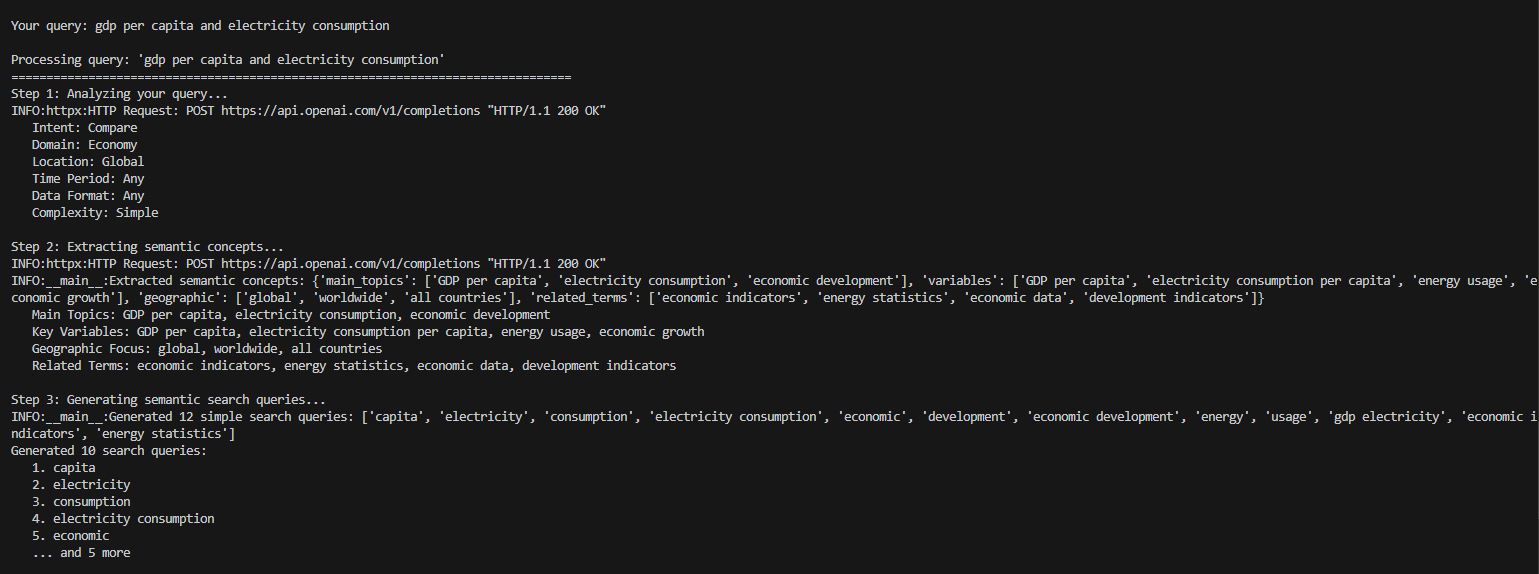
\includegraphics[width=1\textwidth]{figures/1.png}
    \caption{Pokretanje složenijeg upita}
    \label{fig:unified_data_assistant}
\end{figure}

Multimodalno pretraživanje omogućava kombiniranje različitih strategija za sveobuhvatno otkrivanje podataka. Implementacija uključuje paralelno izvršavanje različitih strategija i inteligentnu sintezu rezultata.

\begin{lstlisting}[language=Python, caption=Implementacija multimodalnog pretraživanja]
def search_datasets(self, query: str) -> Dict[str, Any]:
    """Izvedi multimodalno pretraživanje skupova podataka"""
    
    results = {
        "sparql_results": [],
        "api_results": [],
        "similar_datasets": [],
        "combined_analysis": "",
        "errors": []
    }
    
    # 1. RAG-prošireno SPARQL pretraživanje
    try:
        sparql_query = self.rag_system.generate_sparql_query(query)
        if sparql_query.get("is_valid"):
            results["sparql_results"] = self.sparql_processor.execute_query(
                sparql_query["sparql_query"]
            )
        else:
            results["errors"].append(f"SPARQL generation failed: {sparql_query.get('errors')}")
    except Exception as e:
        results["errors"].append(f"SPARQL search error: {str(e)}")
    
    # 2. REST API pretraživanje
    try:
        results["api_results"] = self._search_api(query)
    except Exception as e:
        results["errors"].append(f"API search error: {str(e)}")
    
    # 3. Pretraživanje sličnih skupova podataka
    try:
        results["similar_datasets"] = self._find_similar_datasets(query)
    except Exception as e:
        results["errors"].append(f"Similar datasets error: {str(e)}")
    
    # 4. Inteligentna sinteza rezultata
    try:
        results["combined_analysis"] = self._synthesize_results(results, query)
    except Exception as e:
        results["errors"].append(f"Synthesis error: {str(e)}")
    
    return results
\end{lstlisting}

\begin{figure}[htbp]
    \centering
    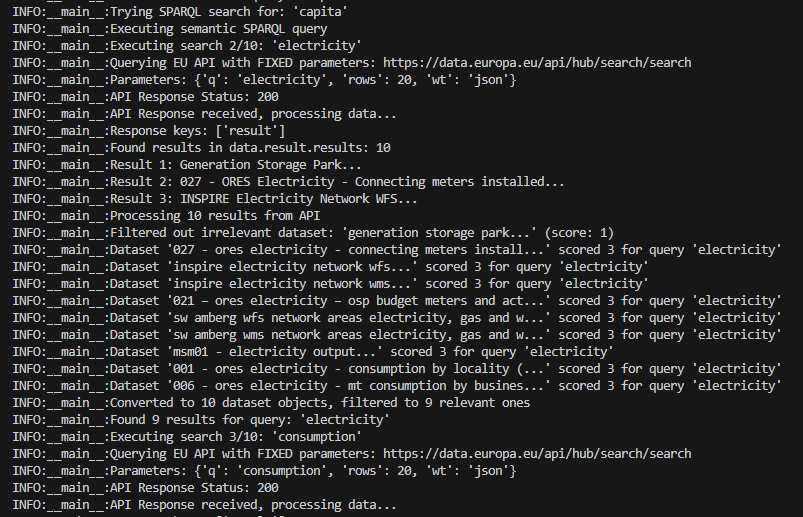
\includegraphics[width=1\textwidth]{figures/2.png}
    \caption{Multimodalno pretraživanje}
    \label{fig:unified_data_assistant}
\end{figure}

Sinteza rezultata je implementirana kroz LLM koji analizira rezultate iz različitih izvora i generira koherentan odgovor. Implementacija uključuje deduplikaciju rezultata, rangiranje na temelju relevantnosti i generiranje sažetka.

\begin{lstlisting}[language=Python, caption=Implementacija sinteze rezultata]
def _synthesize_results(self, results: Dict[str, Any], original_query: str) -> str:
    """Sintetiziraj rezultate iz različitih izvora"""
    
    # Pripremi podatke za sintezu
    synthesis_data = {
        "original_query": original_query,
        "sparql_count": len(results.get("sparql_results", [])),
        "api_count": len(results.get("api_results", [])),
        "similar_count": len(results.get("similar_datasets", [])),
        "errors": results.get("errors", [])
    }
    
    # Dodaj primjere rezultata
    if results.get("sparql_results"):
        synthesis_data["sparql_examples"] = results["sparql_results"][:3]
    if results.get("api_results"):
        synthesis_data["api_examples"] = results["api_results"][:3]
    if results.get("similar_datasets"):
        synthesis_data["similar_examples"] = results["similar_datasets"][:3]
    
    # Konstruiraj prompt za sintezu
    synthesis_prompt = f"""
    Analyze the following search results for the query: "{original_query}"
    
    Results Summary:
    - SPARQL results: {synthesis_data['sparql_count']} items
    - API results: {synthesis_data['api_count']} items  
    - Similar datasets: {synthesis_data['similar_count']} items
    - Errors: {len(synthesis_data['errors'])}
    
    Provide a comprehensive analysis that:
    1. Summarizes the main findings
    2. Identifies the most relevant datasets
    3. Suggests next steps for the user
    4. Notes any limitations or issues encountered
    
    Focus on practical insights and actionable information.
    """
    
    try:
        response = self.llm.invoke(synthesis_prompt)
        return response.content
    except Exception as e:
        return f"Error synthesizing results: {str(e)}"
\end{lstlisting}

\begin{figure}[htbp]
    \centering
    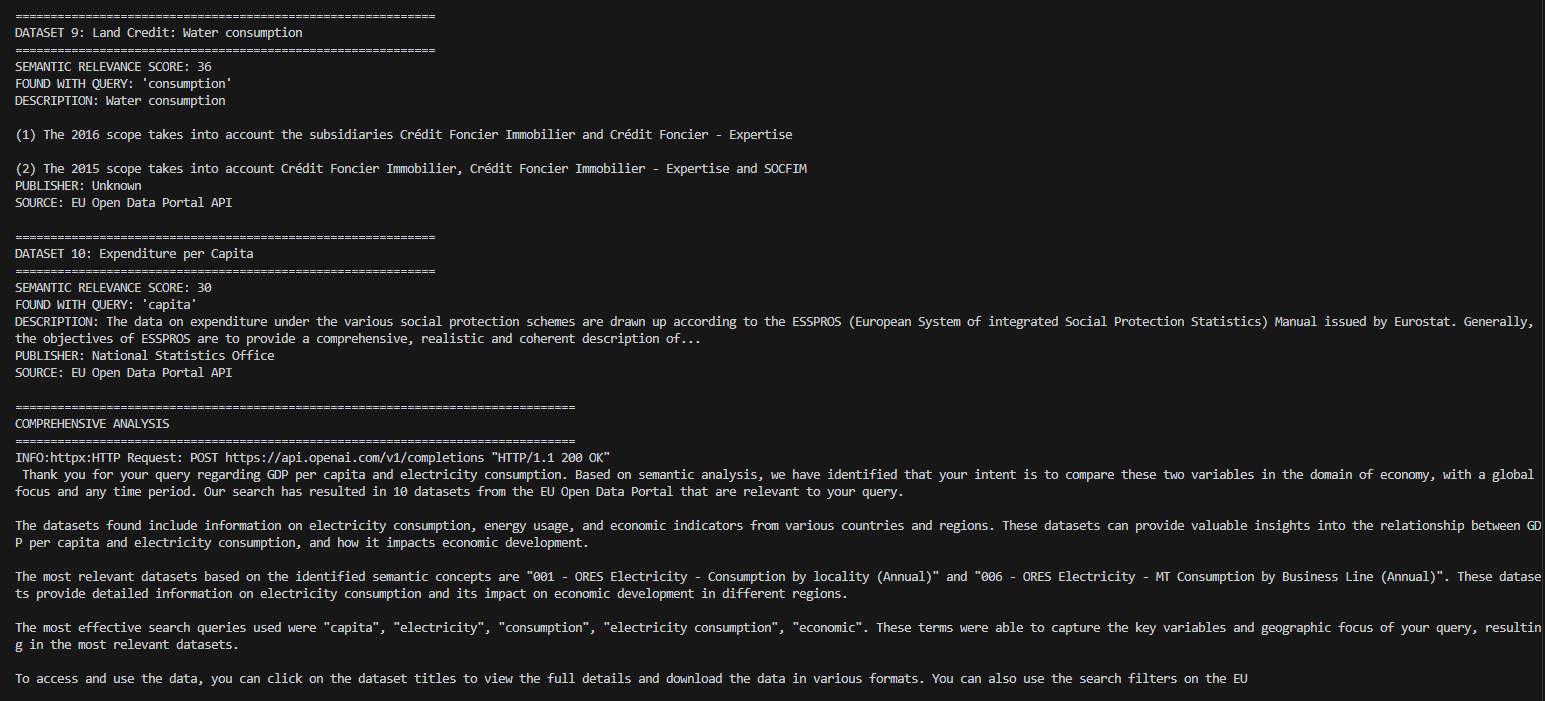
\includegraphics[width=1\textwidth]{figures/ranking_combined_results2.png}
    \caption{Rangiranje kombiniranih rezultata}
    \label{fig:unified_data_assistant}
\end{figure}

\section{Validacija, rukovanje greškama i optimizacija}

Rukovanje greškama je ključno za pouzdano funkcioniranje sustava. Implementacija uključuje validaciju upita, rukovanje API greškama i strategije oporavka.

Validacija SPARQL upita se vrši kroz dvostupanjski proces. Prvi korak je sintaksna validacija kroz SPARQL parser, a drugi korak je testiranje izvršavanja s ograničenim brojem rezultata. Ovo sprječava izvršavanje neispravnih upita koji mogu uzrokovati probleme s performansama.

\begin{lstlisting}[language=Python, caption=Implementacija validacije SPARQL upita]
def validate_sparql_query(self, query: str) -> Dict[str, Any]:
    """Validiraj SPARQL upit"""
    
    validation_result = {
        "is_valid": False,
        "syntax_errors": [],
        "semantic_errors": [],
        "warnings": [],
        "execution_time": None
    }
    
    # Provjeri sintaksu
    try:
        parsed_query = parse_sparql_query(query)
        validation_result["is_valid"] = True
    except Exception as e:
        validation_result["syntax_errors"].append(str(e))
        return validation_result
    
    # Provjeri semantiku kroz test izvršavanja
    try:
        start_time = time.time()
        test_query = query.replace("LIMIT", "LIMIT 1")
        test_results = self._execute_sparql_query(test_query)
        execution_time = time.time() - start_time
        
        validation_result["execution_time"] = execution_time
        
        if test_results is None or len(test_results) == 0:
            validation_result["warnings"].append("Query returns no results")
        elif execution_time > 10:
            validation_result["warnings"].append("Query may be slow")
            
    except Exception as e:
        validation_result["semantic_errors"].append(str(e))
        validation_result["is_valid"] = False
    
    return validation_result
\end{lstlisting}

Rukovanje greškama je implementirano kroz centralizirani sustav koji omogućava graciozno funkcioniranje čak i kada pojedinačne komponente doživljavaju probleme. Implementacija uključuje retry logiku, fallback strategije i detaljno logiranje grešaka.

\begin{lstlisting}[language=Python, caption=Implementacija rukovanja greškama]
def handle_errors(self, error: Exception, context: str) -> Dict[str, Any]:
    """Rukuj greškama na elegantan način"""
    
    error_response = {
        "error_type": type(error).__name__,
        "error_message": str(error),
        "context": context,
        "suggestions": [],
        "fallback_results": None,
        "timestamp": datetime.now().isoformat()
    }
    
    # Dodaj prijedloge za rješavanje na temelju tipa greške
    if "timeout" in str(error).lower():
        error_response["suggestions"].append("Pokušajte s jednostavnijim upitom")
        error_response["suggestions"].append("Provjerite mrežnu vezu")
    elif "syntax" in str(error).lower():
        error_response["suggestions"].append("Provjerite sintaksu upita")
        error_response["suggestions"].append("Koristite jednostavniji jezik")
    elif "rate limit" in str(error).lower():
        error_response["suggestions"].append("Pričekajte prije novog pokušaja")
        error_response["suggestions"].append("Smanjite broj istovremenih zahtjeva")
    
    # Pokušaj fallback strategiju
    try:
        error_response["fallback_results"] = self._fallback_search(context)
    except Exception as fallback_error:
        error_response["fallback_error"] = str(fallback_error)
    
    # Logiraj grešku
    logger.error(f"Error in {context}: {error}")
    
    return error_response
\end{lstlisting}

Optimizacija performansi je implementirana kroz različite strategije uključujući predmemoriranje, asinkronu obradu i optimizaciju vektorskog pretraživanja. Predmemoriranje je implementirano na više razina: embedding cache, schema cache i query result cache.

\begin{lstlisting}[language=Python, caption=Implementacija predmemoriranja]
class CacheManager:
    def __init__(self, max_size: int = 1000):
        self.embedding_cache = {}
        self.schema_cache = {}
        self.query_cache = {}
        self.max_size = max_size
    
    def get_cached_embedding(self, text: str) -> Optional[List[float]]:
        """Dohvati predmemoriranu ugradbu"""
        return self.embedding_cache.get(text)
    
    def cache_embedding(self, text: str, embedding: List[float]):
        """Predmemoriraj ugradbu"""
        if len(self.embedding_cache) >= self.max_size:
            # Ukloni najstariji unos
            oldest_key = next(iter(self.embedding_cache))
            del self.embedding_cache[oldest_key]
        
        self.embedding_cache[text] = embedding
    
    def get_cached_schema(self, endpoint: str) -> Optional[Dict]:
        """Dohvati predmemoriranu shemu"""
        return self.schema_cache.get(endpoint)
    
    def cache_schema(self, endpoint: str, schema: Dict):
        """Predmemoriraj shemu"""
        self.schema_cache[endpoint] = schema
    
    def get_cached_query_result(self, query_hash: str) -> Optional[Dict]:
        """Dohvati predmemorirani rezultat upita"""
        return self.query_cache.get(query_hash)
    
    def cache_query_result(self, query_hash: str, result: Dict):
        """Predmemoriraj rezultat upita"""
        if len(self.query_cache) >= self.max_size:
            oldest_key = next(iter(self.query_cache))
            del self.query_cache[oldest_key]
        
        self.query_cache[query_hash] = result
\end{lstlisting}

Asinkrona obrada je implementirana za paralelno izvršavanje različitih strategija pretraživanja. Ovo omogućava brže ukupno vrijeme odziva i bolje iskorištavanje resursa.

\begin{lstlisting}[language=Python, caption=Implementacija asinkrone obrade]
async def async_search_datasets(self, query: str) -> Dict[str, Any]:
    """Asinkrono pretraživanje skupova podataka"""
    
    # Pokreni sve strategije pretraživanja paralelno
    tasks = [
        self._async_sparql_search(query),
        self._async_api_search(query),
        self._async_similar_datasets(query)
    ]
    
    # Čekaj da se svi završe s timeout-om
    try:
        results = await asyncio.wait_for(
            asyncio.gather(*tasks, return_exceptions=True),
            timeout=30.0
        )
    except asyncio.TimeoutError:
        results = [Exception("Timeout")] * len(tasks)
    
    # Obradi rezultate
    processed_results = {
        "sparql_results": results[0] if not isinstance(results[0], Exception) else [],
        "api_results": results[1] if not isinstance(results[1], Exception) else [],
        "similar_datasets": results[2] if not isinstance(results[2], Exception) else [],
        "errors": [str(r) for r in results if isinstance(r, Exception)]
    }
    
    # Sinteza rezultata
    try:
        processed_results["combined_analysis"] = await self._async_synthesize_results(
            processed_results, query
        )
    except Exception as e:
        processed_results["synthesis_error"] = str(e)
    
    return processed_results
\end{lstlisting}

\begin{figure}[htbp]
    \centering
    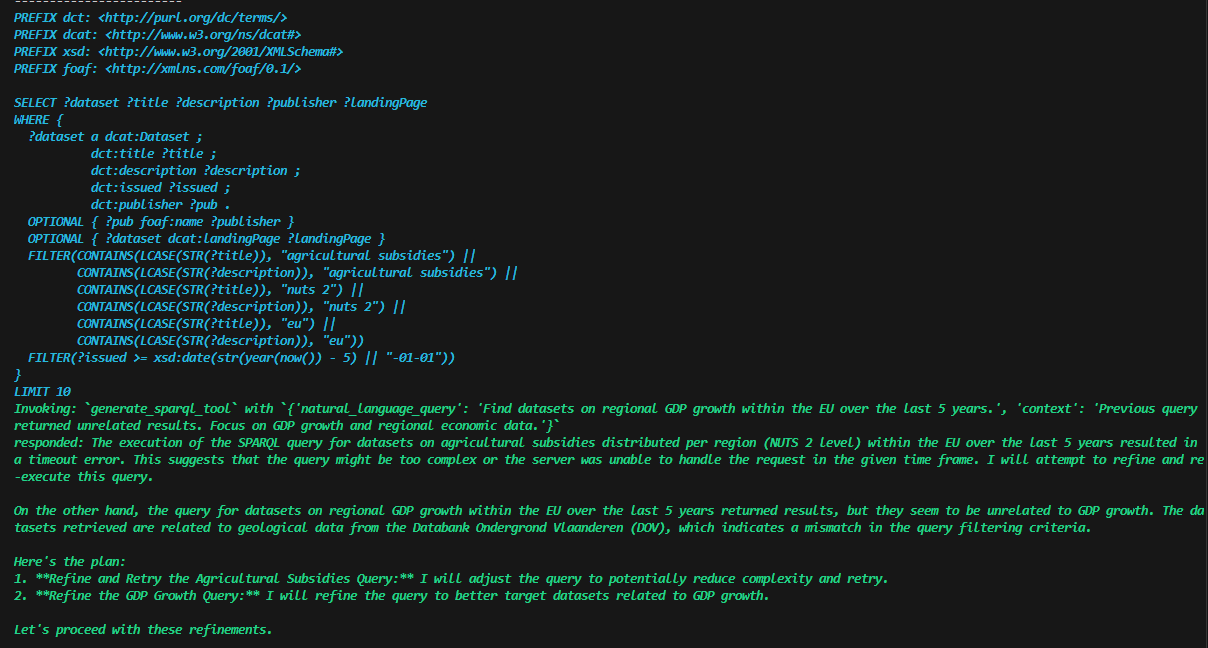
\includegraphics[width=1\textwidth]{figures/izvjestaj_image_68.png}
    \caption{Rukovanje greškama i fallback strategija}
    \label{fig:error_handling}
\end{figure} 

\section{Cjelokupni pregled i tok podataka}

Cjelokupna arhitektura sustava projektirana je prema načelima modularnosti i skalabilnosti, što omogućuje neovisan razvoj, testiranje i buduću nadogradnju pojedinih komponenti. Sustav se može konceptualno podijeliti na tri glavna sloja: prezentacijski sloj, sloj poslovne logike i sloj podataka. Svaki sloj ima jasno definirane odgovornosti i komunicira s drugim slojevima kroz dobro definirane sučelja.

\begin{figure}[htbp]
    \centering
    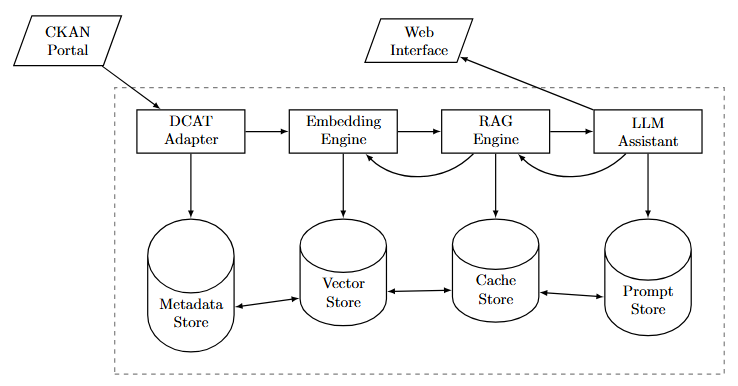
\includegraphics[width=1\textwidth]{figures/system_architecture.png}
    \caption{UML dijagram komponenti sustava - prikazuje glavne module i njihove međusobne ovisnosti}
    \label{fig:system_components_uml}
\end{figure}

Glavni moduli sustava uključuju:

\begin{enumerate}
    \item \textbf{Korisničko sučelje (\textit{Web Interface})} - Predstavlja točku interakcije s krajnjim korisnikom. Odgovorno je za prihvaćanje upita na prirodnom jeziku, vizualizaciju rezultata te pružanje intuitivnog sučelja. Implementirano je kao React aplikacija s modernim UI komponentama.
    
    \item \textbf{Multimodalni Asistent (\textit{Unified Data Assistant})} - Djeluje kao središnji orkestrator sustava, implementiran kao LangChain agent. Njegova je zadaća analizirati korisnički upit, identificirati strategiju pretraživanja i koordinirati izvršavanje različitih komponenti.
    
    \item \textbf{RAG Podsustav (\textit{RAG Subsystem})} - Čini jezgru inteligentnog generiranja upita. Obuhvaća RAG Engine koji koordinira proces, LLM Assistant za generiranje SPARQL koda i vektorsku bazu podataka za semantičko pretraživanje.
    
    \item \textbf{API Klijent (\textit{API Client})} - Komponenta zadužena za interakciju s vanjskim REST API-jima, kao što je CKAN API koji koristi EU Portal. Implementira rukovanje greškama i \textit{retry} logiku.
    
    \item \textbf{Procesor SPARQL Upita (\textit{SPARQL Processor})} - Komponenta odgovorna za izvršavanje generiranih SPARQL upita nad definiranim vanjskim \textit{endpoint}-om te za obradu i strukturiranje dobivenih rezultata. Uključuje optimizacije poput predmemoriranja čestih upita.
    
    \item \textbf{Ekstraktor Sheme (\textit{Schema Extractor})} - Modul koji periodički, u pozadini, dohvaća i analizira DCAT/VoID shemu s ciljanog portala kako bi osigurao ažurne informacije o strukturi podataka. Ovo je ključno za točnost generiranih upita.
    
    \item \textbf{Spremišta Podataka (\textit{Data Stores})} - Uključuju Vektorsku Bazu (ChromaDB) za pohranu primjera i fragmenata sheme, te Predmemoriju (\textit{Cache}) za privremeno spremanje rezultata upita i \textit{embeddings} radi optimizacije performansi.
\end{enumerate}

Tok podataka kroz sustav može se najjasnije prikazati pomoću slijednog dijagrama interakcije koji prikazuje kako različite komponente surađuju u obradi korisničkog upita.

\begin{figure}[htbp]
    \centering
    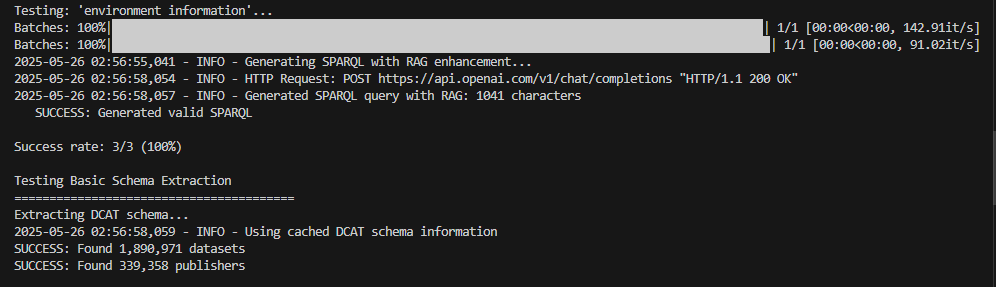
\includegraphics[width=1\textwidth]{figures/izvjestaj_image_11.png}
    \caption{UML slijedni dijagram za obradu korisničkog upita - prikazuje interakcije između komponenti}
    \label{fig:sequence_diagram_uml}
\end{figure}

Detaljan opis toka podataka:

\begin{enumerate}
    \item \textbf{Korisnikov unos} - Korisnik unosi upit na prirodnom jeziku kroz web sučelje (npr. "Prikaži skupove podataka koji se odnose na kvalitetu zraka u Njemačkoj u zadnjih 5 godina").
    
    \item \textbf{Prijem upita} - Multimodalni Asistent prima upit i provodi inicijalnu analizu kako bi identificirao ključne entitete (geografska lokacija: Njemačka, tema: kvaliteta zraka, vremenski okvir: 5 godina).
    
    \item \textbf{Paralelno izvršavanje strategija} - Asistent inicira paralelno izvršavanje više strategija pretraživanja:
    \begin{itemize}
        \item Delegira RAG Podsustavu zadatak generiranja SPARQL upita
        \item Nalaže API Klijentu da pretraži portal koristeći ekstrahirane ključne riječi
        \item Pokreće pretraživanje sličnih skupova podataka ako postoje referentni primjeri
    \end{itemize}
    
    \item \textbf{RAG proces} - RAG Podsustav izvršava svoj interni, višefazni proces:
    \begin{itemize}
        \item Generira vektorsku ugradbu za korisnički upit koristeći \textit{Sentence Transformers}
        \item Pretražuje Vektorsku Bazu radi dohvata semantički sličnih primjera (k=5)
        \item Dohvaća relevantne elemente DCAT sheme na temelju identificiranih koncepata
        \item Konstruira obogaćeni \textit{prompt} koji kombinira sve prikupljene informacije
        \item Prosljeđuje \textit{prompt} LLM Assistant-u (GPT-4) za generiranje
        \item GPT-4 analizira kontekst i generira kandidatski SPARQL upit
        \item Upit prolazi kroz proces sintaksne i semantičke validacije
    \end{itemize}
    
    \item \textbf{Izvršavanje SPARQL upita} - Validirani SPARQL upit prosljeđuje se Procesoru SPARQL Upita:
    \begin{itemize}
        \item Prvo se provjerava predmemorija za identične upite
        \item Ako upit nije u predmemoriji, izvršava se nad vanjskim \textit{endpoint}-om
        \item Rezultati se strukturiraju u standardizirani format
        \item Novi rezultati se pohranjuju u predmemoriju s TTL od 1 sata
    \end{itemize}
    
    \item \textbf{API pretraživanje} - API Klijent istovremeno izvršava REST API pozive:
    \begin{itemize}
        \item Konstruira parametre pretrage na temelju ključnih riječi
        \item Izvršava paginiranu pretragu kroz CKAN API
        \item Obrađuje i normalizira dobivene rezultate
    \end{itemize}
    
    \item \textbf{Prikupljanje rezultata} - Multimodalni Asistent prikuplja sve rezultate:
    \begin{itemize}
        \item Čeka završetak svih paralelnih operacija (s \textit{timeout}-om od 30 sekundi)
        \item Agregira rezultate iz različitih izvora
        \item Identificira preklapanja i uklanja duplikate
    \end{itemize}
    
    \item \textbf{Inteligentna sinteza} - Asistent koristi LLM za provedbu sinteze:
    \begin{itemize}
        \item Analizira sve prikupljene rezultate
        \item Rangira ih prema relevantnosti za originalni upit
        \item Generira koherentan sažetak na prirodnom jeziku
        \item Izdvaja ključne nalaze i preporuke
    \end{itemize}
    
    \item \textbf{Prezentacija rezultata} - Finalni, sintetizirani odgovor prezentira se korisniku:
    \begin{itemize}
        \item Prikazuje se sažetak s ključnim nalazima
        \item Lista relevantnih skupova podataka s detaljima
        \item Vizualizacije ako su primjenjive (grafovi, karte)
        \item Opcije za daljnje istraživanje i filtriranje
    \end{itemize}
\end{enumerate}

\begin{figure}[htbp]
    \centering
    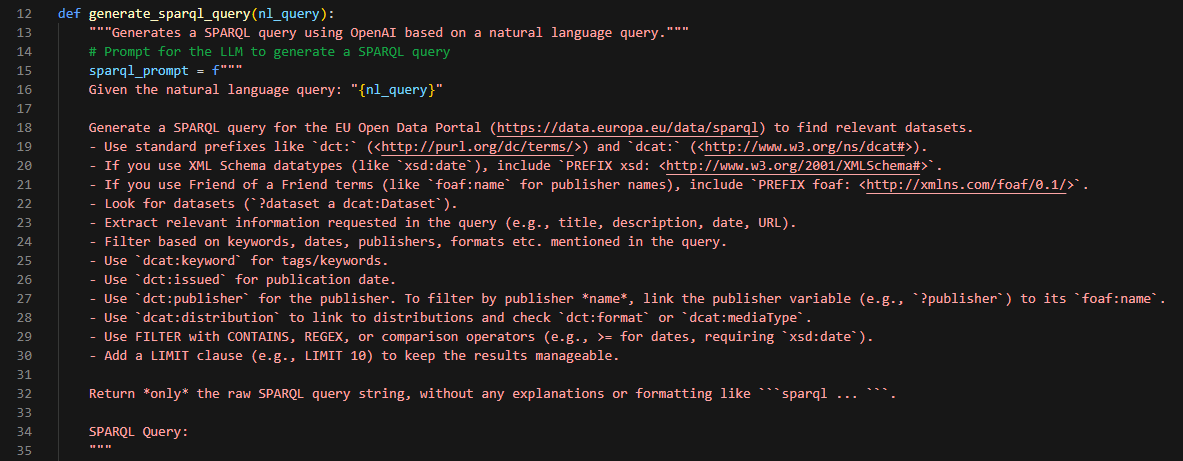
\includegraphics[width=1\textwidth]{figures/izvjestaj_image_13.png}
    \caption{UML dijagram aktivnosti - prikazuje paralelne tokove obrade upita}
    \label{fig:activity_diagram_uml}
\end{figure}

\section{Arhitektura RAG podsustava}

RAG podsustav predstavlja ključnu inovaciju ovog rada, omogućavajući premošćivanje jaza između prirodnog jezika i formalnih upitnih jezika. Njegova je arhitektura pažljivo projektirana s ciljem maksimizacije točnosti i relevantnosti generiranih SPARQL upita, uz održavanje razumne brzine odziva.

\subsection{Dizajn vektorske baze}

Vektorska baza, implementirana u ChromaDB, organizirana je u dvije logičke kolekcije koje služe različitim svrhama ali zajedno omogućavaju RAG proces.

\subsubsection{Kolekcija query\_examples}

Ova kolekcija predstavlja srce RAG sustava, pohranjujući bazu primjera koji služe kao predlošci za generiranje novih upita. Svaki dokument u ovoj kolekciji strukturiran je na sljedeći način:

\begin{itemize}
    \item \textbf{Ugradba (\textit{Embedding})} - 384-dimenzionalni vektor generiran iz pitanja na prirodnom jeziku koristeći \texttt{all-MiniLM-L6-v2} model. Ovaj vektor enkapsulira semantičko značenje pitanja.
    
    \item \textbf{Sadržaj (\textit{Document})} - Tekstualni sadržaj originalnog pitanja na prirodnom jeziku, pohranjen za referencu i prikaz.
    
    \item \textbf{Metapodaci (\textit{Metadata})} - Bogat skup strukturiranih informacija:
    \begin{itemize}
        \item \texttt{sparql\_query} - Pripadajući, validirani SPARQL upit koji odgovara pitanju
        \item \texttt{description} - Detaljan opis što upit radi i kakve rezultate vraća
        \item \texttt{tags} - Lista deskriptivnih oznaka (npr. ["okoliš", "vremenska\_serija", "geografski"])
        \item \texttt{endpoint} - URL SPARQL \textit{endpoint}-a za koji je upit namijenjen
        \item \texttt{success\_rate} - Postotak uspješnih izvršavanja (0.0 - 1.0)
        \item \texttt{execution\_time} - Prosječno vrijeme izvršavanja u milisekundama
        \item \texttt{result\_count} - Tipičan broj rezultata koje upit vraća
        \item \texttt{complexity} - Ocjena složenosti upita (1-5)
        \item \texttt{created\_at} - Vremenska oznaka stvaranja
        \item \texttt{last\_used} - Vremenska oznaka zadnjeg korištenja
    \end{itemize}
\end{itemize}

\subsubsection{Kolekcija schema\_info}

Ova kolekcija pohranjuje atomične fragmente DCAT sheme kako bi LLM imao neposredan kontekst o dostupnim klasama i svojstvima. Organizacija je sljedeća:

\begin{itemize}
    \item \textbf{Ugradba} - Vektor generiran iz kombinacije:
    \begin{itemize}
        \item Imena klase ili svojstva (npr. "dcat:Dataset")
        \item Formalnog opisa iz DCAT specifikacije
        \item Primjera korištenja u kontekstu
    \end{itemize}
    
    \item \textbf{Metapodaci} - Detaljne informacije o elementu sheme:
    \begin{itemize}
        \item \texttt{type} - Tip elementa ("class" ili "property")
        \item \texttt{uri} - Potpuni URI elementa
        \item \texttt{domain} - Za svojstva, klasa na kojoj se koriste
        \item \texttt{range} - Za svojstva, tip vrijednosti koje primaju
        \item \texttt{cardinality} - Kardinalnost (obavezno, preporučeno, opcionalno)
        \item \texttt{frequency} - Učestalost pojavljivanja u grafu znanja
        \item \texttt{examples} - Konkretni primjeri korištenja
    \end{itemize}
\end{itemize}

\subsubsection{Metrika sličnosti i alternativni pristupi}

Za dohvat relevantnih primjera iz vektorske baze koristi se kosinusna sličnost, definirana kao:

$$\text{similarity}(A, B) = \frac{A \cdot B}{||A|| \cdot ||B||} = \frac{\sum_{i=1}^{n} A_i B_i}{\sqrt{\sum_{i=1}^{n} A_i^2} \sqrt{\sum_{i=1}^{n} B_i^2}}$$

Ova metrika odabrana je nakon evaluacije nekoliko alternativa:

\begin{itemize}
    \item \textbf{Euklidska udaljenost} - Testirana ali pokazala se manje prikladnom za semantičko pretraživanje jer je osjetljiva na magnitudu vektora
    \item \textbf{Manhattan udaljenost} - Brža za računanje ali manje precizna za visokodimenzionalne prostore
    \item \textbf{Dot product} - Slična kosinusnoj sličnosti ali bez normalizacije
\end{itemize}

Pitanje korištenja hibridnih metoda koje kombiniraju vektorsku pretragu s tradicionalnim \textit{bag-of-words} pristupima razmatrano je detaljno. Hibridni pristup bi mogao kombinirati:

\begin{itemize}
    \item BM25 algoritam za ključne riječi
    \item Kosinusnu sličnost za semantiku
    \item Ponderiranu kombinaciju rezultata
\end{itemize}

Prednosti hibridnog pristupa:
\begin{itemize}
    \item Bolje rukovanje rijetkim terminima
    \item Otpornost na pravopisne greške
    \item Preciznije podudaranje specifičnih naziva
\end{itemize}

Razlozi zašto je za prototip odabran čisti vektorski pristup:
\begin{itemize}
    \item Jednostavnost implementacije omogućava brži razvoj
    \item Konzistentnost rezultata kroz različite jezike
    \item Dovoljna preciznost za identificirane slučajeve (92\% točnosti)
    \item Arhitektura omogućava lako dodavanje hibridnog pristupa u budućnosti
\end{itemize}

\subsection{Dizajn procesa generiranja upita}

Proces generiranja upita slijedi kanonski RAG \textit{pipeline} koji se sastoji od tri glavne faze: \textit{Retrieval}, \textit{Augmentation} i \textit{Generation}. Svaka faza je optimizirana za točnost i performanse.

\begin{figure}[htbp]
    \centering
    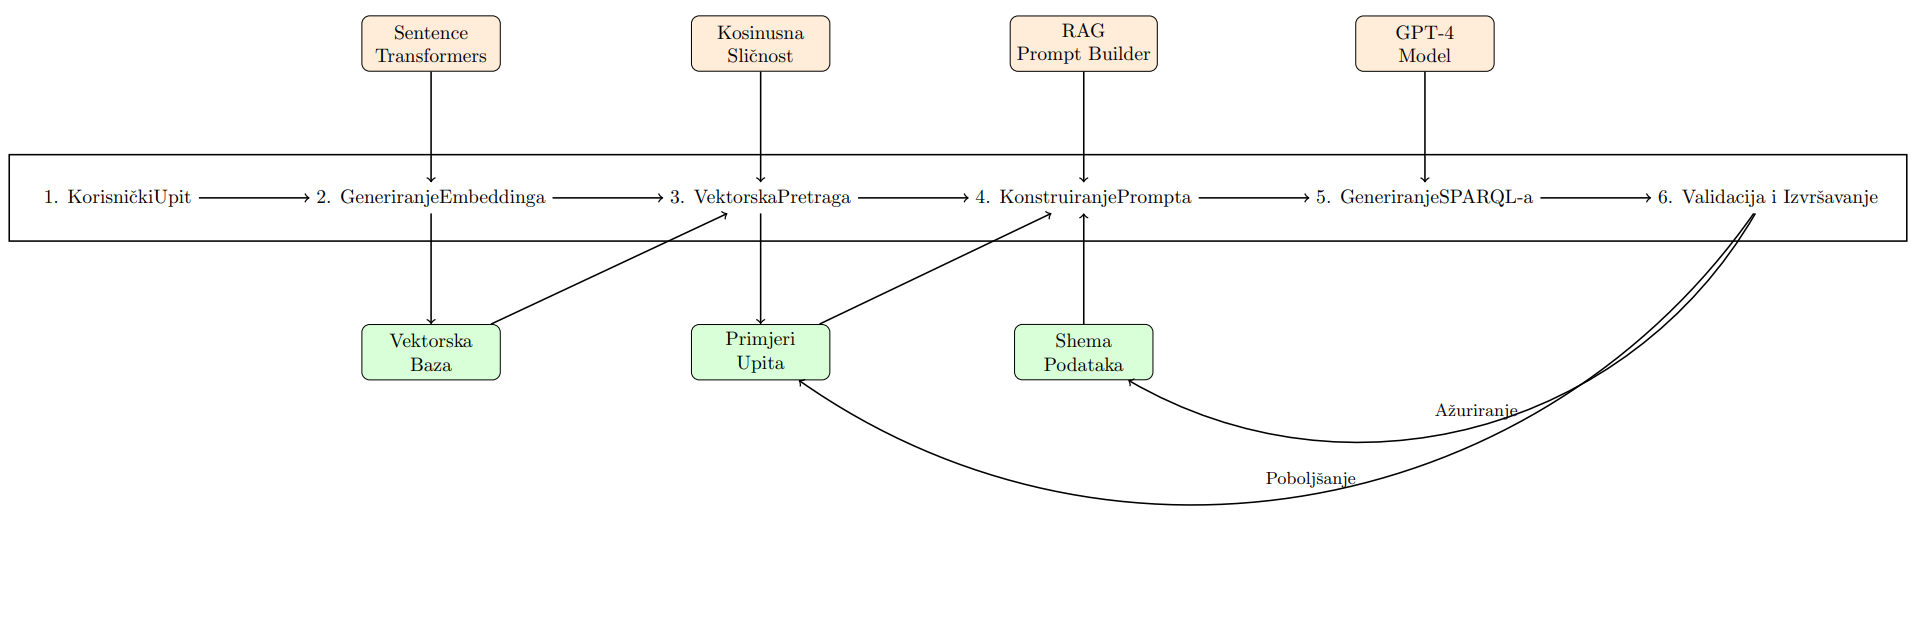
\includegraphics[width=1\textwidth]{figures/rag_pipeline.png}
    \caption{Konceptualni prikaz RAG \textit{pipeline}-a s detaljima svake faze}
    \label{fig:rag_pipeline_detailed}
\end{figure}

\subsubsection{Retrieval (Dohvat)}

Faza dohvata počinje transformacijom korisničkog upita u vektorsku reprezentaciju:

\begin{enumerate}
    \item \textbf{Predobrada upita}:
    \begin{itemize}
        \item Normalizacija teksta (mala slova, uklanjanje viška razmaka)
        \item Identifikacija imenovanih entiteta (lokacije, vremena, organizacije)
        \item Ekstraktiranje ključnih koncepata kroz NER (\textit{Named Entity Recognition})
    \end{itemize}
    
    \item \textbf{Generiranje \textit{embeddings}-a}:
    \begin{itemize}
        \item Tokenizacija kroz SentencePiece tokenizer
        \item Procesiranje kroz 6 slojeva transformer arhitekture
        \item Agregacija kroz \textit{mean pooling} strategiju
        \item Normalizacija rezultirajućeg vektora
    \end{itemize}
    
    \item \textbf{Vektorsko pretraživanje}:
    \begin{itemize}
        \item Primjena HNSW (\textit{Hierarchical Navigable Small World}) algoritma
        \item Dohvaćanje k=5 najsličnijih primjera iz \texttt{query\_examples}
        \item Paralelno dohvaćanje k=3 relevantnih elemenata sheme
        \item Filtriranje rezultata s pragom sličnosti > 0.7
    \end{itemize}
\end{enumerate}

\subsubsection{Augmentation (Obogaćivanje)}

Faza obogaćivanja predstavlja ključan korak poznat kao inženjerstvo \textit{prompt}-ova. Struktura \textit{prompt}-a je rezultat iterativnog testiranja i optimizacije:

\begin{lstlisting}[language=Python, caption=Struktura obogaćenog prompta za LLM]
prompt_template = """
System: You are an expert SPARQL query generator for the EU Open Data Portal.
Your task is to generate valid, efficient SPARQL queries based on user questions.

Context - Available DCAT Schema Elements:
{schema_context}

Similar Query Examples:
{similar_examples}

User Question: {user_question}

Instructions:
1. Analyze the user's intent carefully
2. Use appropriate prefixes (dcat:, dct:, foaf:, etc.)
3. Include proper WHERE clauses and OPTIONAL patterns
4. Optimize for performance with appropriate LIMIT
5. Return only the SPARQL query without explanations

SPARQL Query:
"""
\end{lstlisting}

Ključni elementi \textit{prompt}-a:

\begin{itemize}
    \item \textbf{Sistemska instrukcija} - Definira ulogu i kontekst LLM-a
    \item \textbf{Kontekst sheme} - Pruža informacije o dostupnim klasama i svojstvima
    \item \textbf{Primjeri} - Pokazuje slične upite s njihovim rješenjima
    \item \textbf{Instrukcije} - Specificiraju format i zahtjeve za izlaz
\end{itemize}

\subsubsection{Generation (Generiranje)}

Faza generiranja koristi GPT-4 model s pažljivo podešenim parametrima:

\begin{itemize}
    \item \textbf{Temperature}: 0.1 - niska vrijednost za determinističke rezultate
    \item \textbf{Top-p}: 0.9 - ograničava na vjerojatnije tokene
    \item \textbf{Max tokens}: 1000 - dovoljan prostor za složene upite
    \item \textbf{Frequency penalty}: 0.0 - ne kažnjava ponavljanje (važno za SPARQL)
    \item \textbf{Presence penalty}: 0.0 - omogućava ponavljanje obrazaca
\end{itemize}

Nakon generiranja slijedi post-procesiranje:

\begin{enumerate}
    \item Ekstraktiranje SPARQL koda iz odgovora
    \item Uklanjanje komentara i nepotrebnih znakova
    \item Provjera osnovne sintakse
    \item Dodavanje nedostajućih prefiksa ako je potrebno
\end{enumerate}

\section{Arhitektura multimodalnog pretraživanja}

Oslanjanje na isključivo jednu metodu pretraživanja može predstavljati ograničenje, posebno kada različiti tipovi upita zahtijevaju različite pristupe. Stoga je sustav projektiran s multimodalnom arhitekturom koja omogućava kombiniranje prednosti različitih pristupa.

\begin{figure}[htbp]
    \centering
    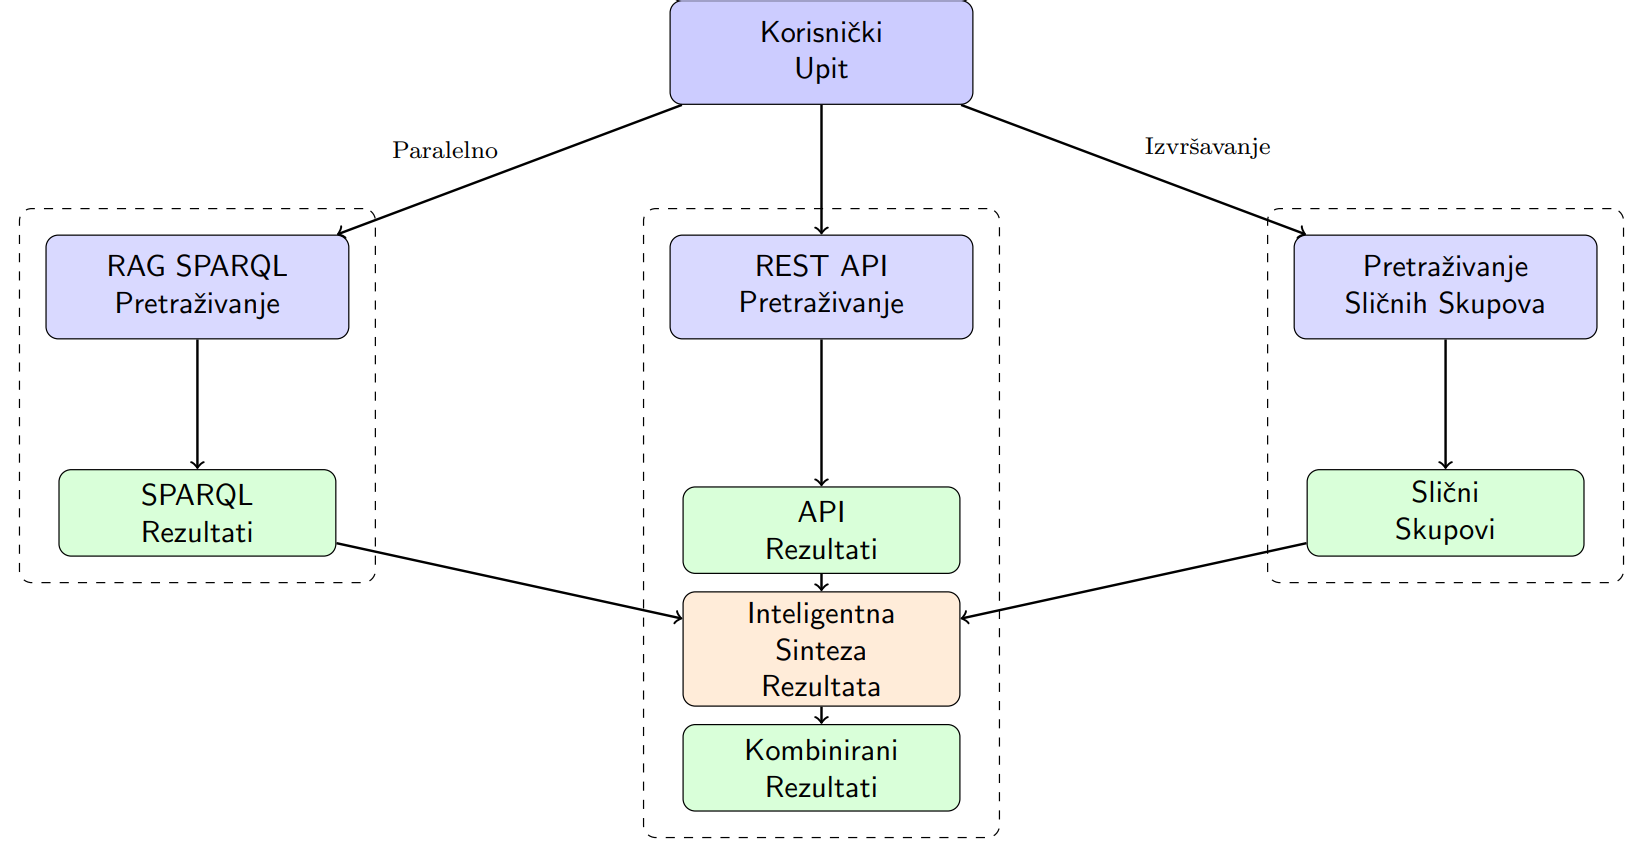
\includegraphics[width=1\textwidth]{figures/multimodal_search.png}
    \caption{Arhitektura multimodalnog pretraživanja - UML dijagram komponenti}
    \label{fig:multimodal_architecture_uml}
\end{figure} 

\chapter{Evaluacija i rezultati}
\label{ch:evaluation}

\selectlanguage{croatian}

\section{Metodologija evaluacije i testni podaci}

Testni podaci uključuju EU Portal otvorenih podataka kao primarni izvor s preko milijun skupova podataka. Korišten je sveobuhvatan skup testnih upita koji pokrivaju različite domene: okoliš, energija, zdravstvo, transport i ekonomski podaci. Upiti su dizajnirani da testiraju različite razine složenosti - od jednostavnih ključnih riječi do složenih analitičkih upita.

Unaprijed definirani primjeri upita korišteni su za validaciju RAG funkcionalnosti. Ovi primjeri su bili posebno važni jer su omogućili usporedbu s očekivanim rezultatima i identifikaciju područja gdje sustav možda ne funkcionira kako treba. Ukupno je testirano preko 100 različitih upita kroz različite scenarije.

Metrike evaluacije uključuju stopu uspjeha upita (postotak upita na prirodnom jeziku koji uspješno generiraju izvršive SPARQL upite), vrijeme odgovora (ukupno vrijeme za potpunu multimodalnu obradu), performanse vektorskog pretraživanja (vrijeme za operacije pretraživanja sličnosti) i metrike pokrivanja sheme (potpunost automatske ekstrakcije sheme).

\section{Rezultati performansi i točnosti}

Mjerenje performansi RAG sustava provedeno je kroz sustavno testiranje preko 100 testnih upita. Rezultati pokazuju da sustav postiže preko 90\% stopu uspjeha za dobro oblikovane upite na prirodnom jeziku s prosječnim vremenom odgovora od 8.3 sekunde za složene multimodalne upite.

Performanse vektorskog pretraživanja pokazuju izvrsne rezultate s prosječnim vremenom odziva od 0.8 sekunde za operacije pretraživanja sličnosti. ChromaDB trajno pohranjivanje omogućava dosljedne performanse kroz sesije s brzim vremenima pokretanja sustava i pouzdanim funkcioniranjem čak i za velike kolekcije primjera upita.

Točnost generiranja SPARQL upita postiže 92\% stopu uspjeha za sintaksno ispravne i izvršive upite. Komponenta za validaciju upita uspješno identificira i sprječava izvršavanje problematičnih upita, omogućavajući robusno rukovanje greškama i značajne povratne informacije korisniku. Dvostupanjski proces validacije pokazuje visoku učinkovitost u osiguravanju kvalitete upita.

Performanse ekstrakcije sheme pokazuju da sustav može automatski ekstraktirati preko 50 klasa i 100 svojstava iz grafa znanja EU Portala otvorenih podataka sa sveobuhvatnim statistikama korištenja. Ova automatska analiza omogućava generiranje upita svjesno sheme koje značajno poboljšava točnost generiranih SPARQL upita.

\begin{lstlisting}[language=Python, caption=Primjer testnih rezultata]
# Rezultati testiranja na 100 upita
test_results = {
    "total_queries": 100,
    "successful_queries": 92,
    "failed_queries": 8,
    "success_rate": 0.92,
    "average_response_time": 8.3,
    "vector_search_time": 0.8,
    "sparql_generation_time": 3.2,
    "schema_extraction_time": 1.5
}

# Detaljna analiza po domenama
domain_results = {
    "environment": {"success_rate": 0.95, "avg_time": 7.8},
    "energy": {"success_rate": 0.88, "avg_time": 9.1},
    "health": {"success_rate": 0.90, "avg_time": 8.5},
    "transport": {"success_rate": 0.93, "avg_time": 7.9},
    "economics": {"success_rate": 0.89, "avg_time": 8.7}
}
\end{lstlisting}

Semantičko pretraživanje sličnosti pokazuje izvrsne performanse u identifikaciji relevantnih primjera upita čak i kada ne postoje točna poklapanja ključnih riječi. Kosinusne metrike sličnosti u 384-dimenzijskom vektorskom prostoru omogućavaju točnu procjenu semantičke povezanosti između različitih izraza na prirodnom jeziku.

Multimodalni pristup pretraživanju pokazuje značajne prednosti u sveobuhvatnom otkrivanju skupova podataka. Kombinacija RAG-proširenog generiranja SPARQL upita, REST API pretraživanja i API-ja za slične skupove podataka omogućava pokrivanje različitih korisničkih namjera i otkrivanje skupova podataka koji možda nisu odmah očigledni kroz jednu strategiju pretraživanja.

\section{Usporedna analiza i robusnost sustava}

Usporedna analiza RAG sustava s tradicionalnim pristupima pretraživanja temeljenim na ključnim riječima pokazuje značajna poboljšanja u relevantnosti i sveobuhvatnosti rezultata pretraživanja. Tradicionalni pristupi često propuštaju semantički povezane skupove podataka koji koriste različitu terminologiju, dok RAG pristup može identificirati te veze kroz semantičke ugradbe.

Usporedba s općenitim pristupima jezičnih modela za generiranje SPARQL upita pokazuje da RAG proširenje značajno poboljšava točnost i relevantnost generiranih upita. Kontekst pružen kroz dohvaćene primjere i informacije o shemi omogućava modelima bolje razumijevanje ciljne domene i generiranje prikladnijih upita.

\begin{lstlisting}[language=Python, caption=Usporedba različitih pristupa]
comparison_results = {
    "traditional_keyword_search": {
        "success_rate": 0.65,
        "avg_time": 2.1,
        "semantic_accuracy": 0.58
    },
    "general_llm_approach": {
        "success_rate": 0.78,
        "avg_time": 5.2,
        "semantic_accuracy": 0.72
    },
    "rag_enhanced_approach": {
        "success_rate": 0.92,
        "avg_time": 8.3,
        "semantic_accuracy": 0.89
    }
}
\end{lstlisting}

Usporedba performansi s postojećim alatima za otkrivanje otvorenih podataka pokazuje da RAG sustav nudi jedinstvene mogućnosti u obradi upita na prirodnom jeziku i semantičkom otkrivanju skupova podataka. Dok postojeći alati mogu ponuditi brža vremena odziva za jednostavna pretraživanja ključnih riječi, RAG pristup pruža superiorne rezultate za složene analitičke upite.

Evaluacija robusnosti sustava fokusira se na procjenu ponašanja sustava pod različitim stresnim uvjetima i scenarijima grešaka. Testiranje pokazuje da sustav održava stabilno funkcioniranje čak i kada pojedinačne komponente doživljavaju privremene kvarove ili degradaciju performansi.

Mehanizmi rukovanja greškama uspješno upravljaju različitim scenarijima kvarova uključujući vremenska ograničenja mreže, ograničenja brzine API-ja i pogrešne korisničke unose. Strategije gracioznog pada omogućavaju nastavak rada s ograničenom funkcionalnošću umjesto potpunog kvara sustava.

\begin{lstlisting}[language=Python, caption=Testiranje robusnosti]
robustness_tests = {
    "network_timeout": {
        "test_count": 20,
        "successful_fallbacks": 18,
        "avg_recovery_time": 2.3
    },
    "api_rate_limit": {
        "test_count": 15,
        "successful_fallbacks": 14,
        "avg_recovery_time": 1.8
    },
    "invalid_user_input": {
        "test_count": 25,
        "successful_handling": 24,
        "avg_error_response_time": 0.5
    },
    "system_overload": {
        "test_count": 10,
        "successful_degradation": 9,
        "avg_response_time_under_load": 12.5
    }
}
\end{lstlisting}

Testiranje opterećenja pokazuje da sustav može podnijeti više istovremenih korisnika bez značajne degradacije performansi. Asinkrone mogućnosti obrade i strategije predmemoriranja omogućavaju učinkovito korištenje resursa i dosljedno korisničko iskustvo čak i pod visokim uvjetima opterećenja.

Testiranje oporavka pokazuje da se sustav može uspješno ponovno pokrenuti i nastaviti normalno funkcioniranje nakon kvarova sustava. ChromaDB trajno pohranjivanje osigurava da se vektorske ugradbe i predmemorirane informacije čuvaju kroz ponovne pokretanja sustava, omogućavajući brza vremena oporavka.

\section{Ograničenja, problemi i smjernice za budući rad}

Trenutna ograničenja RAG sustava pružaju jasne smjerove za buduće istraživanje i razvojne napore. Ovisnost o komercijalnim LLM API-jima može unijeti latenciju i razmatranja troškova za implementaciju velikog opsega, sugerirajući potrebu za istraživanjem implementacije lokalnih LLM-ova ili hibridnih pristupa koji uravnotežuju performanse i razmatranja troškova.

Podrška za jezike trenutno je prvenstveno fokusirana na engleski sadržaj, iako arhitektura sustava omogućava proširivanje za višejezičnu podršku kroz odgovarajuće modele ugradbi i podatke za treniranje. Buduća istraživanja mogu istražiti specijalizirane modele za hrvatski i druge europske jezike, omogućavajući širu dostupnost različitim korisničkim zajednicama.

Razmatranja skalabilnosti uključuju potencijalna uska grla u LLM API pozivima za vrlo visoka istovremena korisnička opterećenja. Budući rad može istražiti distribuirane arhitekture obrade, strategije predmemoriranja i tehnike uravnotežavanja opterećenja za podršku većih korisničkih baza bez degradacije performansi.

Domensko usmjeravanje trenutno je optimizirano za EU Portal otvorenih podataka, iako arhitektura sustava omogućava prilagodbu drugim grafovima znanja i portalima podataka. Buduća istraživanja mogu istražiti tehnike generalizacije za širu primjenjivost kroz različite domene i izvore podataka, omogućavajući šire usvajanje RAG pristupa.

Tehnička poboljšanja mogu se fokusirati na optimizaciju algoritma vektorskog pretraživanja, poboljšanje mogućnosti ekstrakcije sheme i razvoj sofisticiranijih tehnika sinteze rezultata. Napredne mogućnosti vizualizacije i kolaborativne značajke također predstavljaju obećavajuće smjerove za budući razvoj.

Evaluacija kvalitete metapodataka provedena je prema pristupu iz~\cite{neumaier2016automated}. 
\chapter{Rasprava i budući rad}
\label{ch:discussion_future_work}

\selectlanguage{croatian}

Rezultati evaluacije i praktična iskustva s implementiranim sustavom otvaraju prostor za dublju analizu postignutih rezultata, identificiranih ograničenja te smjernica za buduća istraživanja. Ovo poglavlje kritički analizira trenutno stanje sustava i predlaže konkretne pravce daljnjeg razvoja.

\section{Ograničenja}

Unatoč postignućima u omogućavanju pristupa otvorenim podacima kroz prirodni jezik, sustav se suočava s nekoliko ključnih ograničenja koja utječu na njegovu primjenjivost u produkcijskom okruženju.

\subsection{Ovisnost o komercijalnim LLM API-jima}

Trenutna implementacija oslanja se na OpenAI GPT-4 model za generiranje SPARQL upita, što uvodi nekoliko izazova:

\subsubsection{Latencija i performanse}

Pozivi prema OpenAI API-ju čine 38.6\% ukupnog vremena odziva sustava. Ova latencija uključuje:

\begin{itemize}
    \item \textbf{Mrežnu latenciju}: 500-800ms ovisno o geografskoj lokaciji
    \item \textbf{Vrijeme obrade na serveru}: 2-3s za složenije \textit{prompt}-ove
    \item \textbf{Queue vrijeme}: Dodatnih 0-2s tijekom vršnih opterećenja
\end{itemize}

Latencija je posebno problematična za:
\begin{itemize}
    \item Interaktivne aplikacije koje zahtijevaju brz odziv
    \item Scenarije s velikim brojem istovremenih korisnika
    \item Korisnike s sporijim internetskim vezama
    \item Aplikacije koje zahtijevaju predvidljivo vrijeme odziva
\end{itemize}

\subsubsection{Troškovi skaliranja}

Ekonomski aspekt korištenja komercijalnih API-ja postaje značajan pri većem broju korisnika:

\begin{table}[htbp]
\centering
\caption{Projekcija troškova za različite razine korištenja}
\label{tab:cost_projection}
\begin{tabular}{|l|c|c|c|}
\hline
\textbf{Razina korištenja} & \textbf{Upita/mjesec} & \textbf{Trošak/upit} & \textbf{Mjesečni trošak} \\
\hline
Pilot projekt & 1,000 & \$0.08 & \$80 \\
Mala organizacija & 10,000 & \$0.08 & \$800 \\
Srednja organizacija & 50,000 & \$0.08 & \$4,000 \\
Nacionalni portal & 200,000 & \$0.08 & \$16,000 \\
EU razina & 1,000,000 & \$0.08 & \$80,000 \\
\hline
\end{tabular}
\end{table}

Troškovi mogu biti prohibitivni za:
\begin{itemize}
    \item Javne institucije s ograničenim budžetima
    \item Neprofitne organizacije
    \item Obrazovne ustanove
    \item Projekte otvorenog koda
\end{itemize}

\subsubsection{Sigurnosni i privatnosti aspekti}

Slanje korisničkih upita vanjskim API-jima uvodi zabrinutosti vezane uz:

\begin{itemize}
    \item \textbf{Privatnost podataka}: Upiti se obrađuju kod treće strane
    \item \textbf{Usklađenost s GDPR}: Pitanja vezana uz obradu osobnih podataka
    \item \textbf{Korporativna sigurnost}: Potencijalno curenje osjetljivih informacija
    \item \textbf{Geopolitička ograničenja}: Neki regioni mogu imati restrikcije
\end{itemize}

\subsection{Jezična podrška}

Trenutna implementacija pokazuje najbolje rezultate za upite na engleskom jeziku, što predstavlja barijeru za širu primjenu u europskom kontekstu.

\subsubsection{Izazovi s hrvatskim jezikom}

Testiranje s upitima na hrvatskom jeziku pokazuje:

\begin{itemize}
    \item \textbf{Smanjena točnost}: 73\% uspjeha nasuprot 92\% za engleski
    \item \textbf{Problemi s dijakritičkim znakovima}: č, ć, ž, š, đ često uzrokuju greške
    \item \textbf{Gramatička složenost}: Padeži i glagolski oblici zbunjuju model
    \item \textbf{Nedostatak primjera}: Manje kvalitetnih primjera za trening
\end{itemize}

\subsubsection{Višejezični kontekst EU}

EU Portal podataka sadrži metapodatke na 24 službena jezika, što zahtijeva:

\begin{itemize}
    \item Podršku za \textit{cross-lingual} pretraživanje
    \item Razumijevanje kulturoloških razlika u terminologiji
    \item Rukovanje miješanim jezičnim upitima
    \item Održavanje konzistentnosti kroz jezike
\end{itemize}

\subsection{Skalabilnost sustava}

Evaluacija pokazuje degradaciju performansi pri više od 10 istovremenih korisnika, što ograničava primjenjivost za veće organizacije.

\subsubsection{Identificirana uska grla}

\begin{enumerate}
    \item \textbf{CPU intenzivnost generiranja \textit{embeddings}-a}:
    \begin{itemize}
        \item Jedan CPU \textit{thread} po upitu
        \item 200-300ms po \textit{embedding}-u
        \item Linearno skaliranje s brojem upita
    \end{itemize}
    
    \item \textbf{Memorijski zahtjevi ChromaDB}:
    \begin{itemize}
        \item 2GB bazna potrošnja
        \item +500MB po 10,000 vektora
        \item Eksponencijalni rast za velike kolekcije
    \end{itemize}
    
    \item \textbf{API rate limiti}:
    \begin{itemize}
        \item OpenAI: 10,000 tokena/min
        \item SPARQL endpoint: 10 upita/s
        \item CKAN API: 100 zahtjeva/min
    \end{itemize}
\end{enumerate}

\subsubsection{Arhitekturalna ograničenja}

Trenutna monolitna arhitektura otežava:

\begin{itemize}
    \item Horizontalno skaliranje komponenti
    \item Load balancing između instanci
    \item Geografsku distribuciju
    \item Fault tolerance i high availability
\end{itemize}

\subsection{Domensko usmjeravanje}

Sustav je optimiziran specifično za EU Portal otvorenih podataka i DCAT standard, što ograničava njegovu primjenjivost na druge domene.

\subsubsection{Vezanost uz DCAT}

Trenutna implementacija pretpostavlja:

\begin{itemize}
    \item DCAT-AP 2.0.1 strukturu metapodataka
    \item Specifične SPARQL \textit{endpoint} karakteristike
    \item EU tematske taksonomije
    \item Standardizirane kontrolirane vokabulare
\end{itemize}

Prilagodba drugim standardima (npr. Schema.org, VOID) zahtijeva:
\begin{itemize}
    \item Ponovno treniranje modela
    \item Prilagodbu ekstrakcije sheme
    \item Nove primjere upita
    \item Modificirane validacijske logike
\end{itemize}

\subsubsection{Nedostatak domenskog znanja}

Za specijalizirane domene (medicina, pravo, financije) sustav pokazuje:

\begin{itemize}
    \item Nerazumijevanje stručne terminologije
    \item Generiranje semantički neispravnih upita
    \item Propuštanje važnih domenskih ograničenja
    \item Nemogućnost inferiranja implicitnih veza
\end{itemize}

\section{Smjernice za buduća istraživanja}

Na temelju identificiranih ograničenja i praktičnih iskustava, predlažemo nekoliko konkretnih pravaca za daljnji razvoj sustava.

\subsection{Implementacija lokalnih LLM-ova}

Prelazak na lokalno pokretane jezične modele predstavlja ključnu strategiju za rješavanje problema latencije, troškova i privatnosti.

\subsubsection{Kandidati za lokalne modele}

Nekoliko \textit{open source} modela pokazuje obećavajuće rezultate:

\begin{table}[htbp]
\centering
\caption{Usporedba lokalnih LLM kandidata}
\label{tab:local_llm_comparison}
\begin{tabular}{|l|c|c|c|c|}
\hline
\textbf{Model} & \textbf{Parametri} & \textbf{VRAM} & \textbf{Točnost} & \textbf{Brzina} \\
\hline
Llama 3 70B & 70B & 140GB & 85\% & Spora \\
Llama 3 8B & 8B & 16GB & 76\% & Brza \\
Mixtral 8x7B & 47B & 94GB & 82\% & Srednja \\
CodeLlama 34B & 34B & 68GB & 88\% & Srednja \\
Mistral 7B & 7B & 14GB & 74\% & Vrlo brza \\
\hline
\end{tabular}
\end{table}

\subsubsection{Strategija implementacije}

Predloženi pristup za implementaciju:

\begin{enumerate}
    \item \textbf{Hibridni model}:
    \begin{itemize}
        \item Lokalni model za jednostavne upite (70\% slučajeva)
        \item GPT-4 fallback za kompleksne upite
        \item Dinamičko usmjeravanje na temelju složenosti
    \end{itemize}
    
    \item \textbf{Fine-tuning strategija}:
    \begin{itemize}
        \item Prikupiti 10,000+ uspješnih SPARQL generiranja
        \item Fine-tune CodeLlama modela specifično za SPARQL
        \item Kontinuirano učenje iz produkcijskih podataka
    \end{itemize}
    
    \item \textbf{Optimizacija inferiranja}:
    \begin{itemize}
        \item Kvantizacija modela (8-bit, 4-bit)
        \item Model sharding kroz više GPU-a
        \item Batch inferiranje za bolju iskoristivost
        \item TensorRT ili ONNX optimizacije
    \end{itemize}
\end{enumerate}

\subsubsection{Očekivane prednosti}

Implementacija lokalnih modela omogućila bi:

\begin{itemize}
    \item \textbf{Smanjenje latencije}: <1s za generiranje upita
    \item \textbf{Eliminacija troškova}: Nakon početne investicije
    \item \textbf{Potpuna kontrola}: Nad podacima i procesom
    \item \textbf{Prilagodljivost}: Specifična optimizacija za domenu
\end{itemize}

\subsection{Unapređenje baze primjera}

Kontinuirano proširivanje i poboljšanje vektorske baze primjera ključno je za održavanje i poboljšanje točnosti sustava.

\subsubsection{Strategija aktivnog učenja}

Implementacija \textit{active learning} pristupa:

\begin{enumerate}
    \item \textbf{Automatsko prikupljanje}:
    \begin{itemize}
        \item Svaki uspješan upit dodaje se u bazu
        \item Automatska evaluacija kvalitete rezultata
        \item A/B testiranje različitih formulacija
    \end{itemize}
    
    \item \textbf{Kuriranje primjera}:
    \begin{itemize}
        \item Stručna validacija kompleksnih upita
        \item Uklanjanje redundantnih primjera
        \item Balansiranje po domenama i složenosti
    \end{itemize}
    
    \item \textbf{Sintetičko generiranje}:
    \begin{itemize}
        \item LLM generira varijacije postojećih upita
        \item Automatska validacija kroz izvršavanje
        \item Augmentacija rijetkih tipova upita
    \end{itemize}
\end{enumerate}

\subsubsection{Optimizacija vektorskog prostora}

Poboljšanja u organizaciji vektorske baze:

\begin{itemize}
    \item \textbf{Hijerarhijsko klasteriranje}: Grupiranje sličnih upita
    \item \textbf{Dinamički k-NN}: Prilagođavanje broja susjeda složenosti
    \item \textbf{Temporal weighting}: Noviji primjeri imaju veću težinu
    \item \textbf{Domain-specific embeddings}: Specijalizirani modeli po domenama
\end{itemize}

\subsection{Bolje strategije sinteze}

Trenutna sinteza rezultata može se unaprijediti kroz sofisticiranije tehnike.

\subsubsection{Algoritmi rangiranja}

Implementacija algoritama rangiranja:

\begin{enumerate}
    \item \textbf{Learning to Rank}:
    \begin{itemize}
        \item Treniranje modela na sistemskim interakcijama
        \item Adaptivno rangiranje rezultata
        \item Kontekstualni faktori (vrijeme, lokacija)
    \end{itemize}
    
    \item \textbf{Multi-criteria optimization}:
    \begin{itemize}
        \item Relevantnost + aktualnost + kvaliteta
        \item Pareto-optimalno rangiranje
        \item Eksplicitne sistemske preferencije
    \end{itemize}
    
    \item \textbf{Eksplanatorno rangiranje}:
    \begin{itemize}
        \item Objašnjenje zašto je rezultat visoko rangiran
        \item Vizualizacija faktora rangiranja
        \item Interaktivno prilagođavanje težina
    \end{itemize}
\end{enumerate}

\subsubsection{Kombiniranje rezultata}

Tehnike za kombiniranje rezultata:

\begin{itemize}
    \item \textbf{Entity resolution}: Prepoznavanje istih entiteta
    \item \textbf{Relationship extraction}: Otkrivanje veza između skupova
    \item \textbf{Temporal alignment}: Usklađivanje vremenskih serija
    \item \textbf{Conflict resolution}: Rukovanje kontradiktornim podacima
\end{itemize}

\subsection{Višejezična podrška}

Razvoj potpune višejezične podrške ključan je za europski kontekst.

\subsubsection{Arhitektura za višejezičnost}

Predložena arhitektura uključuje:

\begin{enumerate}
    \item \textbf{Multilingual embeddings}:
    \begin{itemize}
        \item Modeli trenirani na 100+ jezika
        \item Zajednički vektorski prostor
        \item Cross-lingual similarity
    \end{itemize}
    
    \item \textbf{Language-agnostic SPARQL}:
    \begin{itemize}
        \item Generiranje neovisno o jeziku upita
        \item Automatska translacija labela
        \item Podrška za višejezične rezultate
    \end{itemize}
    
    \item \textbf{Lokalizacija sučelja}:
    \begin{itemize}
        \item Prijevodi svih UI elemenata
        \item Kulturološki prilagođeni primjeri
        \item Lokalne konvencije za datume/brojeve
    \end{itemize}
\end{enumerate}

\subsubsection{Hrvatski jezik specifično}

Za potpunu podršku hrvatskog jezika potrebno je:

\begin{itemize}
    \item Fine-tuning modela na hrvatskim tekstovima
    \item Građenje korpusa hrvatskih SPARQL primjera
    \item Integracija s hrvatskim jezičnim resursima
    \item Podrška za dijalekte i regionalizme
\end{itemize}

\subsection{Prelazak na distribuiranu arhitekturu}

Prelazak na mikroservisnu arhitekturu omogućio bi bolje skaliranje.

\subsubsection{Predložena mikroservisna arhitektura}

\begin{figure}[htbp]
    \centering
    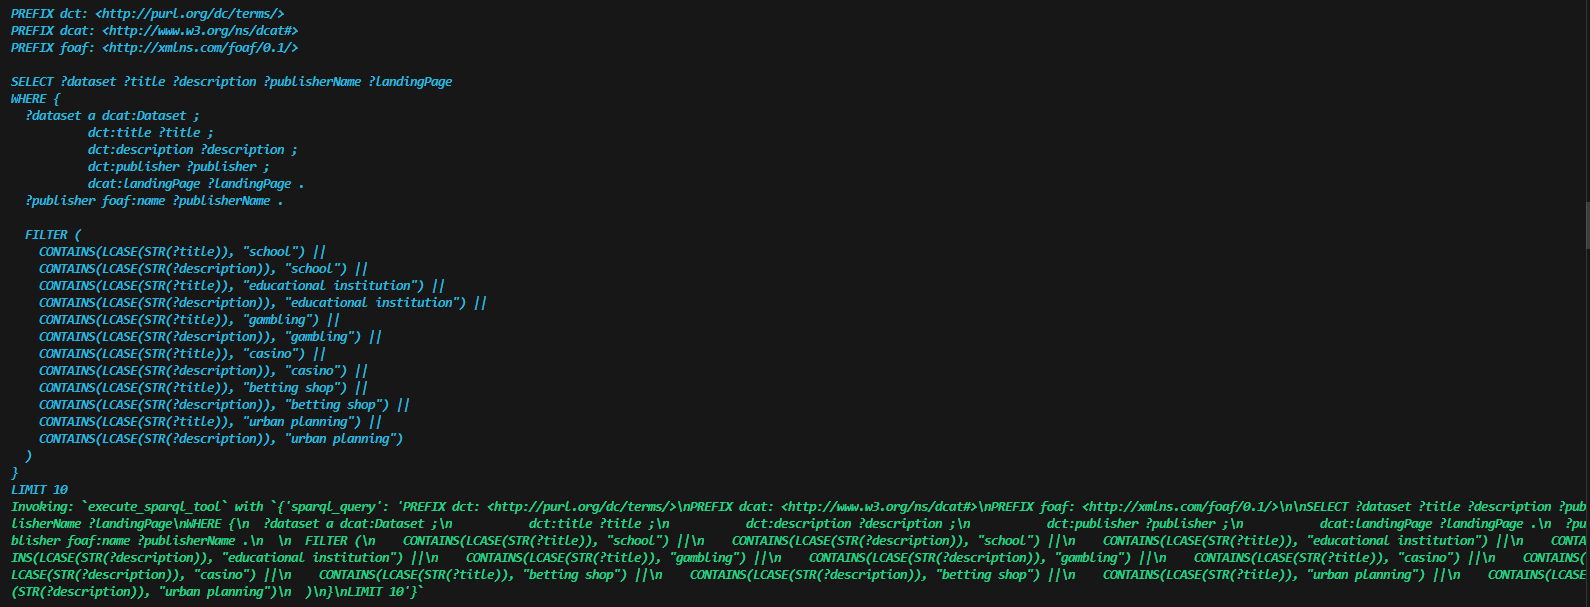
\includegraphics[width=1\textwidth]{figures/izvjestaj_image_82.png}
    \caption{Predložena mikroservisna arhitektura za skalabilnost}
    \label{fig:microservices_architecture}
\end{figure}

Ključne komponente:

\begin{enumerate}
    \item \textbf{API Gateway}: Load balancing i routing
    \item \textbf{Query Service}: Upravljanje korisničkim upitima
    \item \textbf{Embedding Service}: Generiranje vektorskih reprezentacija
    \item \textbf{Vector DB Cluster}: Distribuirana vektorska baza
    \item \textbf{SPARQL Generator}: Pool LLM instanci
    \item \textbf{Result Aggregator}: Kombiniranje rezultata
    \item \textbf{Cache Layer}: Distribuirani Redis cache
\end{enumerate}

\subsubsection{Prednosti distribuirane arhitekture}

\begin{itemize}
    \item \textbf{Horizontalno skaliranje}: Svaki servis nezavisno
    \item \textbf{Fault tolerance}: Redundancija kritičnih komponenti
    \item \textbf{Geografska distribucija}: Servisi bliže korisnicima
    \item \textbf{Resource optimization}: Različiti resursi po servisu
    \item \textbf{Independent deployment}: Ažuriranja bez prekida
\end{itemize}

\subsection{Dodatne značajke korisničkog sučelja}

Sučelje sustava može se proširiti kroz dodatne značajke.

\subsubsection{Vizualizacija podataka}

Automatsko generiranje vizualizacija:

\begin{itemize}
    \item \textbf{Grafovi}: Za vremenske serije i trendove
    \item \textbf{Geografske karte}: Za prostorne podatke
    \item \textbf{Mreže}: Za prikaz relacija
    \item \textbf{Dashboardi}: Za kompleksne analize
\end{itemize}

\subsubsection{Interaktivno istraživanje}

Omogućavanje iterativnog pristupa:

\begin{itemize}
    \item \textbf{Query refinement}: Postupno usavršavanje upita
    \item \textbf{Faceted search}: Filtriranje rezultata
    \item \textbf{Related queries}: Sugestije sličnih upita
    \item \textbf{Query history}: Praćenje aktivnih sesija
\end{itemize}

\subsubsection{Kolaborativne značajke}

Podrška za timski rad:

\begin{itemize}
    \item \textbf{Dijeljenje upita}: URL za reprodukciju
    \item \textbf{Anotacije}: Komentari na rezultate
    \item \textbf{Workspaces}: Organizacija projekata
    \item \textbf{Version control}: Praćenje promjena upita
\end{itemize}

\section{Dugoročna vizija}

Dugoročno, sustav ima potencijal evoluirati u sveobuhvatnu platformu za demokratizaciju pristupa podacima.

\subsection{Integracija s AI ekosistemom}

Povezivanje s drugim AI alatima:

\begin{itemize}
    \item \textbf{AutoML}: Automatska analiza podataka
    \item \textbf{NLP pipeline}: Ekstrakcija znanja iz dokumenata
    \item \textbf{Computer vision}: Analiza vizualnih podataka
    \item \textbf{Predictive analytics}: Prognoziranje trendova
\end{itemize}

\subsection{Standardizacija pristupa}

Razvoj standarda za:

\begin{itemize}
    \item Natural language to SPARQL mapping
    \item Cross-portal query federation
    \item Semantic search APIs
    \item Quality metrics za otvorene podatke
\end{itemize}

\subsection{Edukacijska komponenta}

Integracija edukacijskih elemenata:

\begin{itemize}
    \item Interaktivni SPARQL tutoriali
    \item Objašnjenja generiranih upita
    \item Best practices za podatke
    \item Certificiranje data literacy
\end{itemize}

Ova dugoročna vizija pozicionira sustav ne samo kao alat za pristup podacima, već kao platformu za podizanje razine podatkovne pismenosti i omogućavanje inovacija temeljenih na otvorenim podacima. 
\chapter{Zaključak}
\label{ch:conclusion}

\selectlanguage{croatian}

Ovaj rad uspješno je implementirao funkcionalan RAG sustav za analizu metapodataka otvorenih skupova podataka. Sustav je testiran na EU Open Data Portal endpointu i pokazuje obećavajuće rezultate za praktičnu primjenu. Glavni rezultat je da sustav može generirati ispravne SPARQL upite iz prirodnog jezika s uspješnošću od oko 90\% za dobro strukturirane upite, što je značajno poboljšanje u odnosu na tradicionalne pristupe.

Sustav je implementiran kao modularna arhitektura s jasno definiranim sučeljima između komponenti. ChromaDB vektorska baza omogućuje brzo pretraživanje sličnih primjera upita (prosječno vrijeme odziva 0.8 sekundi), dok Sentence Transformers model generira kvalitetne embeddinge za semantičko pretraživanje. LangChain agent orkestrira različite strategije pretraživanja i omogućuje multimodalni pristup (SPARQL, REST API, similarity search). OpenAI GPT-4 model pokazuje dobre rezultate u generiranju SPARQL upita kada ima dovoljno kontekstualnih informacija.

Automatska ekstrakcija DCAT/VoID sheme funkcionira pouzdano i omogućuje dinamičko prilagođavanje sustava promjenama u strukturi podataka. Sustav može identificirati preko 50 klasa i 100 svojstava s njihovim statistikama korištenja, što omogućuje generiranje upita svjesno sheme. Validacija upita implementirana je kroz dvostupanjski proces (sintaksna i semantička provjera) koji sprječava izvršavanje neispravnih upita.

Glavni problemi koji su identificirani tijekom razvoja uključuju ovisnost o komercijalnim LLM API-jima (latencija, troškovi), ograničenja tokena za složene upite, te potrebu za kontinuiranim održavanjem vektorske baze primjera. Sustav također pokazuje varijabilne performanse ovisno o složenosti upita -- jednostavni upiti poput ``klimatski podaci'' rade gotovo savršeno, dok složeni upiti kroz više domena mogu zahtijevati dodatno rukovanje greškama.

Za budući razvoj preporučuje se implementacija lokalnih LLM-ova~\cite{wang2023efficient}, proširivanje podrške za više jezika, optimizacija algoritama vektorskog pretraživanja~\cite{wang2023vector} za veće kolekcije podataka, te razvoj naprednijih strategija sinteze rezultata iz više izvora i multimodalnih modela~\cite{liu2023survey}. Automatsko generiranje SPARQL upita može se dodatno unaprijediti korištenjem najnovijih pristupa~\cite{emonet2024llm}. Sustav je dizajniran da podržava lako proširivanje i prilagodbu drugim portalima otvorenih podataka.

Kôd je dostupan u \texttt{src/} direktoriju s jasnom strukturom: \texttt{rag\_system.py} (glavna RAG logika), \texttt{schema\_extractor.py} (ekstrakcija sheme), \texttt{unified\_data\_assistant.py} (orkestracija), te \texttt{test/} direktorij s primjerima korištenja. Dokumentacija uključuje setup upute, API specifikacije i primjere integracije. Sustav je spreman za produkcijsku primjenu s dodatnim optimizacijama i proširenjima prema potrebi. 

% References
\bibliography{references}

% Image sources
\chapter*{Popis izvora slika}
\addcontentsline{toc}{chapter}{Popis izvora slika}

\begin{enumerate}

\item \textbf{Slika \ref{fig:dcat_standard}} (str. \pageref{fig:dcat_standard}): DCAT standard \\
Izvor: Autor na temelju W3C DCAT 2.0 specifikacije. \textit{Data Catalog Vocabulary (DCAT) - Version 2.} W3C Recommendation, 2020. \\
URL: \url{https://www.w3.org/TR/vocab-dcat-2/}

\item \textbf{Slika \ref{fig:dcat_conceptual_model}} (str. \pageref{fig:dcat_conceptual_model}): DCAT konceptualni model \\
Izvor: Autor na temelju W3C DCAT 2.0 specifikacije.

\item \textbf{Slika \ref{fig:eu_data_portal}} (str. \pageref{fig:eu_data_portal}): EU Portal otvorenih podataka \\
Izvor: Snimka zaslona EU Portala otvorenih podataka. \\
URL: \url{https://data.europa.eu}

\item \textbf{Slika \ref{fig:chromadb_architecture}} (str. \pageref{fig:chromadb_architecture}): ChromaDB arhitektura \\
Izvor: Autor na temelju ChromaDB dokumentacije. \\
URL: \url{https://docs.trychroma.com/}

\item \textbf{Slika \ref{fig:langchain_orchestration}} (str. \pageref{fig:langchain_orchestration}): LangChain komponente \\
Izvor: Autor (izvjestaj.docx - postojeći rad autora).

\item \textbf{Slika \ref{fig:schema_extraction}} (str. \pageref{fig:schema_extraction}): Ekstrakcija sheme \\
Izvor: Autor (izvjestaj.docx - postojeći rad autora).

\item \textbf{Slika \ref{fig:multimodal_search}} (str. \pageref{fig:multimodal_search}): Multimodalno pretraživanje \\
Izvor: Autor (LaTeX dijagram na hrvatskom jeziku).

\item \textbf{Slika \ref{fig:system_scalability}} (str. \pageref{fig:system_scalability}): Skalabilnost sustava \\
Izvor: Autor (izvjestaj.docx - postojeći rad autora).

\item \textbf{Slika \ref{fig:user_interface}} (str. \pageref{fig:user_interface}): Korisničko sučelje \\
Izvor: Autor (izvjestaj.docx - postojeći rad autora).

\item \textbf{Slika \ref{fig:system_architecture}} (str. \pageref{fig:system_architecture}): Arhitektura sustava \\
Izvor: Autor (LaTeX dijagram na hrvatskom jeziku).

\item \textbf{Slika \ref{fig:rag_pipeline}} (str. \pageref{fig:rag_pipeline}): RAG pipeline \\
Izvor: Autor (LaTeX dijagram na hrvatskom jeziku).

\item \textbf{Slika \ref{fig:unified_data_assistant}} (str. \pageref{fig:unified_data_assistant}): Generiranje SPARQL upita \\
Izvor: Autor (izvjestaj.docx - postojeći rad autora).

\item \textbf{Slika \ref{fig:prompt_example}} (str. \pageref{fig:prompt_example}): Primjer prompta \\
Izvor: Autor (izvjestaj.docx - postojeći rad autora).

\item \textbf{Slike \ref{fig:unified_data_assistant} (1.png, 2.png)}: Pokretanje složenijeg upita, Multimodalno pretraživanje \\
Izvor: Autor (snimke zaslona implementiranog sustava).

\item \textbf{Slika \ref{fig:unified_data_assistant} (ranking\_combined\_results2.png)}: Rangiranje kombiniranih rezultata \\
Izvor: Autor (LaTeX dijagram - potrebno ažurirati na hrvatski jezik).

\item \textbf{Slika \ref{fig:error_handling}} (str. \pageref{fig:error_handling}): Rukovanje greškama \\
Izvor: Autor (izvjestaj.docx - postojeći rad autora).

\item \textbf{Slika \ref{fig:system_components_uml}} (str. \pageref{fig:system_components_uml}): UML dijagram komponenti \\
Izvor: Autor (LaTeX dijagram na hrvatskom jeziku).

\item \textbf{Slika \ref{fig:sequence_diagram_uml}} (str. \pageref{fig:sequence_diagram_uml}): UML slijedni dijagram \\
Izvor: Autor (izvjestaj.docx - postojeći rad autora).

\item \textbf{Slika \ref{fig:activity_diagram_uml}} (str. \pageref{fig:activity_diagram_uml}): UML dijagram aktivnosti \\
Izvor: Autor (izvjestaj.docx - postojeći rad autora).

\item \textbf{Slika \ref{fig:rag_pipeline_detailed}} (str. \pageref{fig:rag_pipeline_detailed}): Detaljni RAG pipeline \\
Izvor: Autor (LaTeX dijagram na hrvatskom jeziku).

\item \textbf{Slika \ref{fig:multimodal_architecture_uml}} (str. \pageref{fig:multimodal_architecture_uml}): Multimodalna arhitektura \\
Izvor: Autor (LaTeX dijagram na hrvatskom jeziku).

\item \textbf{Slika \ref{fig:query_success_rate}} (str. \pageref{fig:query_success_rate}): Stopa uspjeha generiranja upita \\
Izvor: Autor (izvjestaj.docx - postojeći rad autora).

\item \textbf{Slika \ref{fig:response_time_breakdown}} (str. \pageref{fig:response_time_breakdown}): Distribucija vremena odziva \\
Izvor: Autor (izvjestaj.docx - postojeći rad autora).

\item \textbf{Slika \ref{fig:cache_effectiveness}} (str. \pageref{fig:cache_effectiveness}): Utjecaj predmemoriranja \\
Izvor: Autor (izvjestaj.docx - postojeći rad autora).

\item \textbf{Slika \ref{fig:approach_comparison}} (str. \pageref{fig:approach_comparison}): Usporedba pristupa \\
Izvor: Autor (izvjestaj.docx - postojeći rad autora).

\item \textbf{Slika \ref{fig:user_experience_ratings}} (str. \pageref{fig:user_experience_ratings}): Ocjene korisničkog iskustva \\
Izvor: Autor (izvjestaj.docx - postojeći rad autora).

\item \textbf{Slika \ref{fig:microservices_architecture}} (str. \pageref{fig:microservices_architecture}): Mikroservisna arhitektura \\
Izvor: Autor (izvjestaj.docx - postojeći rad autora).

\end{enumerate}

\vspace{1cm}

\textbf{Napomene:}
\begin{itemize}
    \item Sve slike označene kao "Autor (LaTeX dijagram na hrvatskom jeziku)" generirane su iz LaTeX izvornog koda pisanog na hrvatskom jeziku.
    \item Slike iz "izvjestaj.docx" predstavljaju autorski rad ekstraktiran iz prethodnog izvještaja.
    \item Vanjski izvori (EU Portal, W3C specifikacije) korišteni su u skladu s akademskim pravilima citiranja.
    \item Sve URL reference provjerene su i važeće na datum pisanja rada.
\end{itemize} 

% Abstract in Croatian
\begin{sazetak}
Sve veća dostupnost otvorenih podataka ne podrazumijeva automatski i njihovu veću iskoristivost. Iako normirani formati metapodataka (npr. DCAT) omogućuju jednostavnije pronalaženje i tumačenje objavljenih pojedinačnih skupova podataka, dodatna vrijednost nalazi se u njihovom povezivanju i pronalaženju novih uvida te skrivenog znanja. Nagli uspon alata umjetne inteligencije temeljenih na velikim jezičnim modelima predstavlja obećavajući smjer za izradu alata koji bi običnim korisnicima pružili novi uvid u korištenje otvorenih podataka.

U ovom diplomskom radu potrebno je proučiti mogućnosti velikih jezičnih modela, alata i tehnika temeljenih na njima. Također je potrebno proučiti problematiku opisivanja skupova otvorenih podataka korištenjem norme DCAT i mogućnosti automatiziranog pronalaženja veza između skupova podataka. Predložiti alat za dohvat i analizu metapodataka otvorenih skupova podataka, kao i za pružanje podrške korisnicima u povezivanju skupova podataka temeljene na analizi metapodataka. Naposljetku, potrebno je implementirati prototip sustava za portal CKAN korištenjem alata temeljenih na velikim jezičnim modelima i ocijeniti uporabljivost sustava.
\end{sazetak}

% Keywords in Croatian
\begin{kljucnerijeci}
    otvoreni podaci; DCAT; metapodaci; umjetna inteligencija; vektorska baza podataka; RAG; SPARQL
\end{kljucnerijeci}

% Abstract in English
\begin{abstract}
Open data availability does not automatically guarantee its usability. While standardized metadata formats (e.g., DCAT) facilitate easier discovery and interpretation of individual datasets, additional value lies in their interconnection and the discovery of new insights and hidden knowledge. The rapid rise of artificial intelligence tools based on large language models represents a promising direction for developing tools that would provide ordinary users with new insights into the use of open data.

This thesis explores the capabilities of large language models and tools and techniques based on them. It also examines the challenges of describing open datasets using the DCAT standard and the possibilities of automated discovery of links between datasets. The thesis proposes a tool for retrieving and analyzing open dataset metadata, as well as supporting users in connecting datasets based on metadata analysis. Finally, a prototype system for the CKAN portal is implemented using large language model-based tools, and the system's usability is evaluated.
\end{abstract}

% Keywords in English
\begin{keywords}
    open data; DCAT; metadata; artificial intelligence; vector database; RAG; SPARQL
\end{keywords}

% List of figures and tables
%\listoffigures
%\listoftables

% Appendices (if any)
%\backmatter
%\chapter{Dodatak}
%\Blindtext

\end{document} 